
\setcounter{chapter}{4}

\chapter{Challenges of ambiguity in word meaning}
\label{c:gg}

\begin{figure}[t]
  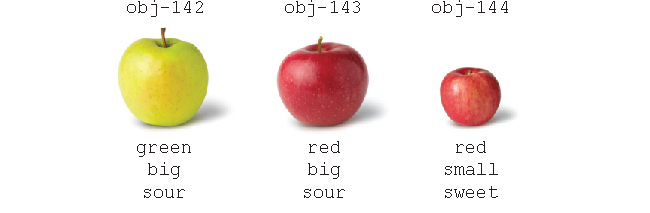
\includegraphics[scale=0.85]{figures/sgg-example-perception-apples}
  \caption{Example of a simulated world perception. Objects have a
    temporary identifier for establishing reference (\texttt{obj-142},
    \texttt{obj-143}, etc.) and are characterized by a set of
    categories (\texttt{green}, \texttt{big}, etc).}
  \label{f:sgg-example-perception-apples}
\end{figure}

Next we investigate a variety of models that take the Naming Game from
the previous chapter one step further in complexity. Rather than
having the world provide unique categories that then directly become
the meanings underlying an utterance, objects in the world are now
characterized by a set of properties, as shown in the exemplary
context in Figure \ref{f:sgg-example-perception-apples}. Unlike in the
Naming Game, object labels such as \texttt{obj-142}, \texttt{obj-143},
etc. can not be used as meanings, because they do not remain the same
for objects across contexts -- instead they serve as a ``pointer''
that serves as a reference to an object during a game. For setting
objects apart, each of them has a set of properties such as
\texttt{green}, \texttt{big}, and so on. As discussed in Section
\ref{s:representing-linguistic-knowlede}, these properties can be seen
as \emph{categories}, \emph{attributes}, or \emph{features}, and they
are essentially unstructured symbols that are part of the world and
that are thus automatically shared between the agents of the
population. We will call them categories for the remainder of this
thesis.



In order to draw attention to one of such objects, the speaker needs
to construct a set of categories that allow the hearer to distinguish
the object from all other objects in the context. This process is
called \emph{conceptualization} (see Section
\ref{s:saussure-to-peirce}) and the resulting category set serves as
the meaning that is then verbalized by the speaker. For example in the
scene of Figure \ref{f:sgg-example-perception-apples}, the category
\texttt{green} can be used to distinguish \texttt{obj-142} from all
other objects, because no other object has this property. Similarly,
the categories \texttt{small} and \texttt{sweet} are each sufficient
to discriminate \texttt{obj-144} from the rest. However, only the
combined meanings \texttt{red} $\wedge$ \texttt{big} and \texttt{red}
$\wedge$ \texttt{sour} distinguish \texttt{obj-143} from the other
objects, because each single category of this object is also found in
one of the others.


This additional conceptualization layer creates a variety of further
ambiguities, and the degree of these uncertainties depends on the
nature of word representations (see Section
\ref{s:nature-of-form-meaning-couplings} on page
\pageref{s:nature-of-form-meaning-couplings}). Most importantly, a hearer
perceiving a novel form can not know directly which meaning to
adopt. For example, upon hearing ``fabesi'' for \texttt{obj-144} in
the scene of Figure \ref{f:sgg-example-perception-apples}, the hearer
can infer from the context that the word does not mean \texttt{red}
(because \texttt{obj-143} is also red), but he is left with the
uncertainty whether the speaker meant \texttt{small} or
\texttt{sweet}. Furthermore, when word meanings are not restricted to
single categories but can be structured, the number of potential
meanings multiplies because any discriminating combination of
categories is a meaning candidate. Finally, when utterances are
allowed to contain multiple words, there is the additional uncertainty
in guessing which word carries which meaning. And from the perspective
of a single agent, it is undecidable which words contributed to
communicative failure when updating word scores at the end of a game.\\

\noindent In this chapter we will analyze a number of strategies for dealing
with these challenges. After briefly introducing the world simulation
that we are going to use in Section \ref{s:sgg-world-simulator}, we
will investigate four lexicon formation models that differ in two
aspects. First, whether word meanings are restricted to single
categories (unstructured word meanings) or whether forms can be
associated to sets of categories (structured word meanings). And
second, whether agents can use multiple words to express a meaning
(multi-word utterances) or whether
they use only a single word (single-word utterances):\\

\centerline{\small\renewcommand{\arraystretch}{1.5}
  \begin{tabular}{rp{2cm}p{2.2cm}}
    & single-word utterances & multi-word utterances \\
    unstructured meanings (single categories)  & Section \ref{s:sgg-sw-unstructured} & Section \ref{s:sgg-mw-unstructured} \\
    structured meanings (category sets) & Section \ref{s:sgg-sw-structured} & Section \ref{s:sgg-mw-structured} 
  \end{tabular}}


\section{A simple world simulator}
\label{s:sgg-world-simulator}


A simple world simulation provides our agents with artificial
perceptions such as illustrated in Figure
\ref{f:sgg-example-perception-apples}. In each interaction, a set of
objects $O=\{o_1, o_2, \dots\}$, each containing a number of distinct
categories, is randomly created and perceived by both the speaker and
hearer. The number of objects in a context $O$ is randomly chosen to
be in the range $cs_{min} \leq |O| \leq cs_{max}$. The set of
available categories in the world $C := \{c_1, c_2, \dots\}$ is
constant throughout an experimental run and each object $o \subset C$
consists of a fixed number $|o|$ of categories from $C$ that are
randomly drawn. The world simulator guarantees that no two objects in
a context have the same set of categories.


Throughout this and the next chapter, by default the number of available categories
$|C|$ is 15, the number of categories per object $|o|$ is 10, the
minimum number of objects in a context $cs_{min}$ is 2, and the
maximum context size $cs_{max}$ is 5. An example context that was
created with these parameters is shown below:

\centerline{\footnotesize\sffamily
  \begin{tabular}{l|l}
    object & categories \\
    \hline
    \texttt{obj-53} & \texttt{c-4  c-2  c-6  c-12  c-9  c-1  c-14  c-5  c-3  c-15  }\\
    \texttt{obj-54} & \texttt{c-10  c-5  c-11  c-9  c-3  c-2  c-8  c-6  c-7  c-14  }\\
    \texttt{obj-55} & \texttt{c-7  c-5  c-6  c-2  c-15  c-8  c-10  c-13  c-4  c-3  }\\
    \texttt{obj-56} & \texttt{c-10  c-2  c-4  c-7  c-1  c-5  c-6  c-3  c-9  c-13  }\\
  \end{tabular}}




\section{Single words for single categories}
\label{s:sgg-sw-unstructured}

We first look at how populations of agents can agree a set of names
for single categories in language games with single- word
utterances. The additional challenge for reaching coherence compared
to the Naming Game will be that agents will associate word forms to
multiple meanings, in addition to connecting multiple forms to the
same meanings.


\subsection{Conceptualization, interpretation \& the interplay with
  words}
\label{s:sgg-sw-unstructured-conceptualization}

Most of the strategies for representing and processing words, for
playing a language game and for learning are identical to those in the
Naming Game (see Section \ref{s:ng-strategies} on page
\pageref{s:ng-strategies}). Here, we will only discuss the
differences.

\inparagraph{Lexicon representation} Form meaning representations are
represented in an identical way as in the Naming Game. The set of
possible word meanings ${\cal M}$ amounts to the set of available
categories in the world $C$.

\inparagraph{Conceptualization} Given the topic chosen by the speaker
and the perceived context, the conceptualization process computes all
categories that part of the topic but not of the other objects. For
example with this context \\

\centerline{\footnotesize\sffamily
  \begin{tabular}{l|l}
    object & categories \\
    \hline
    \texttt{obj-3696} & \texttt{c-3  c-15  c-11  c-2  c-6  c-10  c-14  c-4  c-13  c-8  }\\
    \texttt{obj-3697} & \texttt{c-1  c-9  c-13  c-7  c-3  c-8  c-4  c-11  c-6  c-10  }\\
    \texttt{obj-3698} & \texttt{c-2  c-14  c-10  c-11  c-15  c-12  c-5  c-6  c-13  c-8  } \\   
    \multicolumn{2}{l}{}
  \end{tabular}}

\noindent and \texttt{obj-3697} as the topic, conceptualization comes
up with three alternative meanings: \texttt{c-7}, \texttt{c-1} and
\texttt{c-9}. When no such category can be found, then
conceptualization fails, the speaker signals a communicative failure,
and the next interaction starts. 

\begin{figure}[t]
  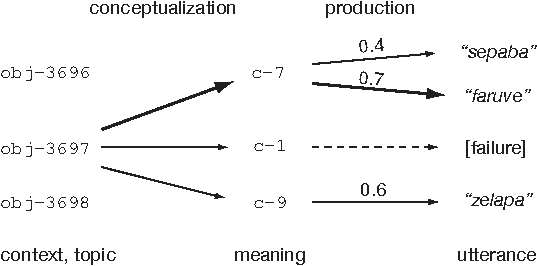
\includegraphics[scale=0.8]{figures/sgg-semiotic-network-production}
  \caption{Example of a semiotic network in
    production. Conceptualization constructs three different meanings,
    and the lexicon is applied independently to each of them. The path
    that leads to the utterance with the highest word score is drawn
    with a thicker line. }
  \label{f:sgg-semiotic-network-production}
\end{figure}

\inparagraph{Production and the interplay with conceptualization} As
in the Naming Game, the speaker looks up his lexicon for all words
that have the category resulting from conceptualization as their
meaning and from these selects the word with the highest association
score. The difference, however, is that conceptualization often
results in multiple meanings. The lexicon is looked up for each of
them in parallel, and in the end the meaning-utterance combination
with the highest word score is selected. Figure
\ref{f:sgg-semiotic-network-production} illustrates this approach. The
lexicon is independently applied to the three different meanings
\texttt{c-7}, \texttt{c-1} and \texttt{c-9}, and while this agent does
not have a word for \texttt{c-1}, he knows one word for \texttt{c-9}
and two words for \texttt{c-7}. Of all these utterances, ``faruve'' is
then chosen by the speaker because it involved the word with the
highest score of 0.7.

As a consequence of this, it is the lexicon that `selects' the
meanings that are verbalized, which we will later see is a good
strategy. By using the scores of the involved words as a criterion for
which meaning to choose, the speaker increases his chance to be
understood, because higher word scores also mean that the population
reached more consensus about how to name a particular category.


\inparagraph{Invention} Only when production completely fails,
i.e. the speaker does not have a word for any of the conceptualized
meanings, a new word is created for a randomly chosen meaning and
production is retried again.

\begin{figure}[t]
  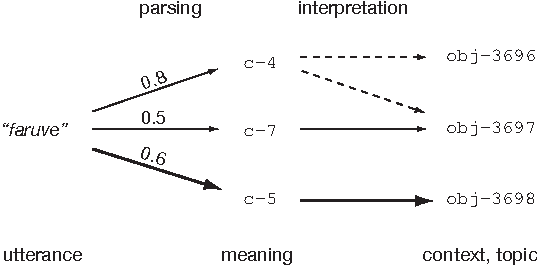
\includegraphics[scale=0.8]{figures/sgg-semiotic-network-parsing}
  \caption{Example of a semiotic network in parsing. The lexicon of
    this agent contains three different meanings for ``faruve'', which
    are each interpreted independently. The path with the highest word
    score that leads to a single interpreted topic is drawn with a
    thicker line. }
  \label{f:sgg-semiotic-network-parsing}
\end{figure}

\inparagraph{Parsing} The hearer retrieves all words from his own
lexicon that match the utterance. Each of these meanings is then
independently interpreted in the context.

\inparagraph{Interpretation and the interplay with parsing} A meaning
is interpreted in the context by retrieving all objects that share the
category. When multiple objects found for a meaning (and thus the
parsed meaning does not discriminate an object from the rest), then
interpretation for that particular meaning fails. Again, this process
is interconnected with lexicon application. Out of the successful
interpretations, the where the involved form-meaning association has
the highest score is eventually selected. 

An example of this is shown in Figure
\ref{f:sgg-semiotic-network-parsing}. Although the association from
``faruve'' to \texttt{c-4} has the highest score, it is not selected
because the semantic interpretation of \texttt{c-4} results in two
different referents. Instead, the next highest word with the meaning
\texttt{c-5} is chosen, yielding \texttt{obj-3698} as the topic
interpreted by the hearer. Through this, the context constrains
ambiguity in the lexicon by excluding words meanings that are not in
line with the current scene.

\inparagraph{Recovery from failure \& adoption} Three cases are
distinguished when an interaction fails. First, when the hearer could
not come up with a topic (either because he did not know the word or
because interpretation returned multiple objects), then he
re-conceptualizes the scene for the topic pointed at by the speaker
and for each resulting meaning stores an association to the form heard
in his lexicon. Second, when the hearer pointed to the wrong object
(and is consequently corrected by the speaker), then he checks whether
another path in his processing led to the correct topic. For example
in Figure \ref{f:sgg-semiotic-network-parsing}, the alternative path
``faruve'' $\longrightarrow$ \texttt{c-7} $\longrightarrow$
\texttt{obj-3697} would have resulted in the topic intended by the
speaker but was not chosen because the score of the involved word was
not the highest. In such a case, nothing happens and this particular
path is treated specially in consolidation (below). And third, when
the hearer pointed to the wrong object and no other correct path in
processing existed, then the hearer also re-conceptualizes the scene
and adds new words for all the resulting meanings to his lexicon
(except those for which already an association to the form heard
exists).

\begin{figure}[t]
  
\centerline{\footnotesize\renewcommand{\arraystretch}{1.3}{
\begin{tabular}{llllllllc}
  \# & speaker & topic & meaning & utterance & hearer & meaning & topic & success? \\
  \hline
500 & agent 6 & \texttt{obj-1783} &  &  & agent 2 &  &  & no \\
501 & agent 1 & \texttt{obj-1785} & \texttt{c-6} & \textit{``ziraxo''} & agent 8 & \texttt{c-5} & \texttt{obj-1785} & yes \\
502 & agent 1 & \texttt{obj-1787} & \texttt{c-15} & \textit{``wimure''} & agent 9 & \texttt{c-13} & \texttt{obj-1788} & no \\
503 & agent 6 & \texttt{obj-1789} & \texttt{c-15} & \textit{``namuvo''} & agent 5 & \texttt{c-3} &  & no \\
504 & agent 8 & \texttt{obj-1792} &  &  & agent 9 &  &  & no \\
505 & agent 10 & \texttt{obj-1797} & \texttt{c-14} & \textit{``xazapo''} & agent 5 & \texttt{c-14} & \texttt{obj-1797} & yes \\
506 & agent 8 & \texttt{obj-1799} & \texttt{c-9} & \textit{``kugoma''} & agent 9 & \texttt{c-9} & \texttt{obj-1799} & yes \\
507 & agent 7 & \texttt{obj-1803} &  &  & agent 4 &  &  & no \\
508 & agent 7 & \texttt{obj-1805} & \texttt{c-6} & \textit{``ziraxo''} & agent 4 & \texttt{c-6} & \texttt{obj-1805} & yes \\
509 & agent 3 & \texttt{obj-1806} & \texttt{c-8} & \textit{``namuvo''} & agent 9 &  &  & no \\
510 & agent 2 & \texttt{obj-1810} & \texttt{c-1} & \textit{``bikuse''} & agent 4 & \texttt{c-12} &  & no \\
511 & agent 6 & \texttt{obj-1812} &  &  & agent 4 &  &  & no \\
512 & agent 10 & \texttt{obj-1817} & \texttt{c-8} & \textit{``gubawo''} & agent 5 & \texttt{c-4} &  & no \\
513 & agent 8 & \texttt{obj-1819} & \texttt{c-7} & \textit{``vatage''} & agent 10 & \texttt{c-7} & \texttt{obj-1819} & yes \\
514 & agent 6 & \texttt{obj-1822} &  &  & agent 7 &  &  & no \\
 \\\end{tabular}}}


%%% Local Variables: 
%%% mode: latex
%%% TeX-master: "../phd-thesis"
%%% End: 

  \caption{Overview of 15 consecutive interactions from game 500
    on. It shows the agents that are interacting, the topic chosen by
    the speaker, the conceptualized meaning that was chosen, the
    utterance, the meaning parsed by the hearer together with the
    interpreted topic, and whether the agents reached communicative
    success.}
  \label{f:sgg-sw-unstructured-trace}
\end{figure}

\begin{figure}[t]
  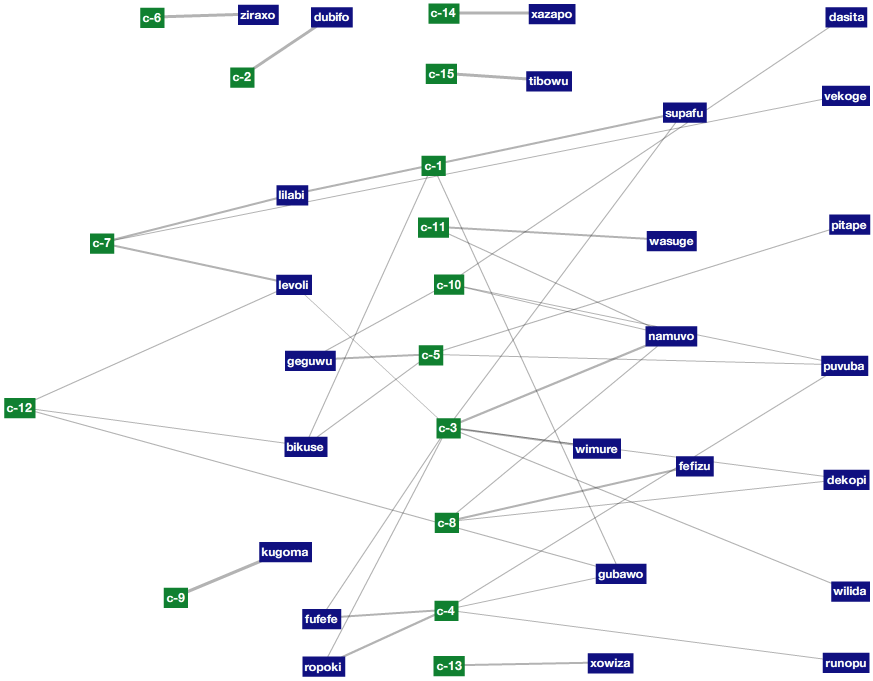
\includegraphics[width=\textwidth]{figures/sgg-sw-unstructured-lexicon-1500}
  \caption{Network representation of the complete lexicon of the first
    agent in the population after 1500 interactions. Each line
    represents a word in the lexicon of the agent and connects the
    meaning of the word with its form. The line widths denote the
    strength of the association. }
  \label{f:sgg-sw-unstructured-lexicon-1500}
\end{figure}

\inparagraph{Consolidation} The consolidation strategy is very similar
to the Naming Game. After a failed interaction, the score of the word
used is lowered in score. After a success, the score of the
responsible word increased and those of words with competing forms are
laterally inhibited. The parameters for this update are also the same,
with $\Delta_s=0.1$, $\Delta_f=-0.1$ and $\Delta_i=-0.2$. 

However, there two differences. First, since now there is also the
possibility that multiple meanings are associated to the same form,
they also need to be reduced, which is done using the same lateral
inhibition as for competing forms. Second, when the hearer pointed to
the wrong topic but another path in his processing lead to the correct
topic (as described above), then the score of the word involved is
updated as if the interaction would have been a success (i.e. the
score of the word is increased and words with competing forms or
meanings are inhibited).


\subsection{Dynamics and strategies for reducing ambiguity}
\label{s:sgg-sw-unstructed-strategies}


Figure \ref{f:sgg-sw-unstructured-trace} shows an example of 15
consecutive language games in a population of 10 agents that follow
the strategies described in the previous section. There are a variety
of differences to the Naming Game. First, it can happen that the
speaker is not able to produce an utterance because conceptualization
fails (for example in interaction 500). Second, even when the hearer
is able to parse an utterance, it can happen that non of the resulting
meanings yield a unique object in the context (e.g interaction
503). Third, even when the hearer is able to infer a referent, it
might still be a different one than intended by the speaker
(e.g. interaction 502). And fourth, even when speaker and hearer reach
communicative success, their understanding of the word used might
still be different. For example in interaction 501, the speaker
conceptualizes \texttt{obj-1785} as \texttt{c-6}. The hearer parses
the utterance as \texttt{c-5}, but by chance this gets interpreted as
the same object as intended speaker and consequently, both agents
assume that they used the word ``ziraxo'' correctly and will update
word scores accordingly.



These additional uncertainties are clearly reflected in early states
of the agents' lexicons. Figure
\ref{f:sgg-sw-unstructured-lexicon-1500} shows a snapshot of the
lexicon of the first agent in the population after 1500
interactions. Although this agent has already settled on the forms for
some categories (mostly at the top of the graph), many meanings in
that lexicon are not only linked to multiple forms as before, but
because hearers adopt multiple meanings for forms in the case of
failure, there are also many forms that are connected to multiple
meanings. In order to establish an unambiguous one-to-one mapping of
single forms to single meanings, alignment dynamics need to reduce
these competing forms and meanings over the course of many
interactions.

\startfiguregroup


\begin{figure}[t]
  
{\footnotesize\renewcommand{\arraystretch}{1.5}
\begin{tabular}{@{}p{1.2cm}|p{1.6cm}@{}p{0.8cm}@{}|p{1.6cm}@{}p{0.8cm}@{}|p{1.6cm}@{}p{0.8cm}@{}|p{1.6cm}@{}p{0.8cm}@{}}
meaning & agent 1 &  & agent 2 &  & agent 3 &  & agent 4 & \\
\hline
\texttt{c-1}&\textit{``lilabi''}


\textit{``bikuse''}


\textit{``gubawo''}


\textit{``supafu''}
&0.50

0.20

0.30

0.40&\textit{``dasita''}


\textit{``lazixe''}


\textit{``xowiza''}


\textit{``lilabi''}
&0.40

0.30

0.30

0.20&\textit{``dasita''}


\textit{``lilabi''}


\textit{``bixina''}


\textit{``xowiza''}
&0.50

0.50

0.10

0.40&\textit{``bixina''}


\textit{``namuvo''}


\textit{``vugumi''}


\textit{``lazixe''}


\textit{``bikuse''}


\textit{``ropoki''}


\textit{``runopu''}


\textit{``dekopi''}


\textit{``supafu''}
&0.60

0.30

0.30

0.30

0.20

0.10

0.30

0.30

0.10\\
\hline
\texttt{c-2}&\textit{``dubifo''}
&1.00&\textit{``wimure''}


\textit{``supafu''}


\textit{``fuxefa''}


\textit{``tigasi''}


\textit{``dubifo''}
&0.50

0.50

0.10

0.10

0.50&\textit{``sipuva''}


\textit{``dubifo''}
&0.30

0.50&\textit{``wimure''}


\textit{``vekoge''}


\textit{``vugumi''}


\textit{``lazixe''}


\textit{``dutiru''}


\textit{``dubifo''}
&0.40

0.40

0.50

0.50

0.10

0.50\\
\hline
\texttt{c-3}&\textit{``wimure''}


\textit{``levoli''}


\textit{``fufefe''}


\textit{``namuvo''}


\textit{``supafu''}


\textit{``ropoki''}


\textit{``dekopi''}


\textit{``wilida''}
&0.50

0.30

0.30

0.40

0.30

0.30

0.20

0.20&\textit{``wimure''}


\textit{``vatage''}


\textit{``dekopi''}


\textit{``miwupa''}


\textit{``ropoki''}


\textit{``fuxefa''}


\textit{``bikuse''}


\textit{``puvuba''}


\textit{``namuvo''}
&0.50

0.50

0.50

0.50

0.50

0.50

0.40

0.30

0.40&\textit{``pitape''}


\textit{``gubawo''}


\textit{``miwupa''}


\textit{``geguwu''}


\textit{``sekero''}
&0.50

0.30

0.20

0.60

0.30&\textit{``levoli''}


\textit{``wimure''}


\textit{``vugumi''}


\textit{``supafu''}


\textit{``tigasi''}


\textit{``lazixe''}


\textit{``geguwu''}
&0.50

0.40

0.30

0.30

0.10

0.20

0.20\\
\end{tabular}}

%%% Local Variables: 
%%% mode: latex
%%% TeX-master: "../phdbook"
%%% End: 

  \caption{Forms associated to 3 different meanings by the first four
    agents of a population of 10 after 1500 interactions.}
  \label{f:sgg-sw-unstructured-lexicon-meanings-1500}
\end{figure}

\begin{figure}[t]
  
{\renewcommand{\arraystretch}{1.5}
\begin{tabular}{@{}p{1.2cm}|p{1.6cm}@{}p{0.8cm}@{}|p{1.6cm}@{}p{0.8cm}@{}|p{1.6cm}@{}p{0.8cm}@{}|p{1.6cm}@{}p{0.8cm}@{}}
form & agent 1 &  & agent 2 &  & agent 3 &  & agent 4 & \\
\hline
\textit{``levoli''}&\texttt{c-12}


\texttt{c-7}


\texttt{c-3}
&0.30

0.40

0.30&\texttt{c-12}
&0.40&&&\texttt{c-11}


\texttt{c-7}


\texttt{c-3}


\texttt{c-4}
&0.50

0.50

0.50

0.40\\
\hline
\textit{``lilabi''}&\texttt{c-1}


\texttt{c-7}
&0.50

0.50&\texttt{c-1}
&0.20&\texttt{c-1}
&0.50&\texttt{c-7}
&0.40\\
\hline
\textit{``dubifo''}&\texttt{c-2}
&1.00&\texttt{c-5}


\texttt{c-2}
&0.10

0.50&\texttt{c-2}
&0.50&\texttt{c-11}


\texttt{c-2}
&0.40

0.50\\
\end{tabular}}

%%% Local Variables: 
%%% mode: latex
%%% TeX-master: "../phdbook"
%%% End: 

  \caption{Meanings associated to 3 different forms by the first four
    agents of a population of 10 after 1500 interactions.}
  \label{f:sgg-sw-unstructured-lexicon-forms-1500}
\end{figure}

\stopfiguregroup

\startfiguregroup

\begin{figure}[t]
  
{\footnotesize\renewcommand{\arraystretch}{1.5}
\begin{tabular}{@{}p{1.2cm}|p{1.6cm}@{}p{0.8cm}@{}|p{1.6cm}@{}p{0.8cm}@{}|p{1.6cm}@{}p{0.8cm}@{}|p{1.6cm}@{}p{0.8cm}@{}}
meaning & agent 1 &  & agent 2 &  & agent 3 &  & agent 4 & \\
\hline
\texttt{c-1}&\textit{``lilabi''}
&1.00&\textit{``lilabi''}
&1.00&\textit{``lilabi''}
&1.00&\textit{``lilabi''}
&1.00\\
\hline
\texttt{c-2}&\textit{``dubifo''}
&1.00&\textit{``dubifo''}
&1.00&\textit{``dubifo''}
&0.80&\textit{``dubifo''}
&1.00\\
\hline
\texttt{c-3}&\textit{``geguwu''}
&1.00&\textit{``geguwu''}
&0.90&\textit{``geguwu''}
&1.00&\textit{``geguwu''}
&1.00\\
\end{tabular}}

%%% Local Variables: 
%%% mode: latex
%%% TeX-master: "../phd-thesis"
%%% End: 

  \caption{Forms associated to 3 different meanings by the first four
    agents of a population of 10 after 5000 interactions.}
  \label{f:sgg-sw-unstructured-lexicon-meanings-5000}
\end{figure}

\begin{figure}[t]
  
{\renewcommand{\arraystretch}{1.5}
\begin{tabular}{@{}p{1.2cm}|p{1.6cm}@{}p{0.8cm}@{}|p{1.6cm}@{}p{0.8cm}@{}|p{1.6cm}@{}p{0.8cm}@{}|p{1.6cm}@{}p{0.8cm}@{}}
form & agent 1 &  & agent 2 &  & agent 3 &  & agent 4 & \\
\hline
\textit{``geguwu''}&\texttt{c-3}
&1.00&\texttt{c-3}
&1.00&\texttt{c-3}
&1.00&\texttt{c-3}
&1.00\\
\hline
\textit{``lilabi''}&\texttt{c-1}
&1.00&\texttt{c-1}
&1.00&\texttt{c-1}
&1.00&\texttt{c-1}
&1.00\\
\hline
\textit{``dubifo''}&\texttt{c-2}
&1.00&\texttt{c-2}
&1.00&\texttt{c-2}
&1.00&\texttt{c-2}
&1.00\\
\end{tabular}}

%%% Local Variables: 
%%% mode: latex
%%% TeX-master: "../phdbook"
%%% End: 

  \caption{Meanings associated to 3 different forms by the first four
    agents of a population of 10 after 5000 interactions.}
  \label{f:sgg-sw-unstructured-lexicon-forms-5000}
\end{figure}

\stopfiguregroup


Once more, Figure \ref{f:sgg-sw-unstructured-lexicon-meanings-1500}
compares the forms associated by four agents in the population to
three categories after 1500 interactions. Because the number of
potential word meanings (15 categories) is bigger than in the Naming
Game in the previous chapter (10 objects), and because due to the
uncertainty in meaning the same forms become associated to multiple
categories, there are more competing forms for each category in the
lexicons (compare Figure \ref{f:ng-lexicon-250}, page
\pageref{f:ng-lexicon-250}). Analogously, competing meanings for
three forms in the lexicons of the same four agents are shown in
Figure \ref{f:sgg-sw-unstructured-lexicon-forms-1500}. The degree
of competition between meanings is less than for forms, as we also see
later on. Finally, partial lexicons at the end of the alignment
process are shown in Figure
\ref{f:sgg-sw-unstructured-lexicon-meanings-5000} and
\ref{f:sgg-sw-unstructured-lexicon-forms-5000}. Competing forms and
meaning have been completely eliminated and unambiguous mappings from
single categories to single forms have been established.


\startfiguregroup

\begin{figure}[t]
  \gnuplotfigure{figures/sgg-sw-unstructured-word-form-scores-c-2}
  \caption{Evolution of words with the meaning \texttt{c-2} in the
    population. Each line shows for a single form the corresponding
    word scores averaged over all agents that connect the form to
    \texttt{c-2}. }
  \label{f:sgg-sw-unstructured-word-form-scores-c-2}
\end{figure}

\begin{figure}[t]
  \gnuplotfigure{figures/sgg-sw-unstructured-word-meaning-scores-dubifo-}
  \caption{Evolution of words with the form ``dubifo'' in the
    population. Each line shows for a single meaning the corresponding
    word scores averaged over all agents that associate this meaning
    to ``dubifo''. }
  \label{f:sgg-sw-unstructured-word-meaning-scores-dubifo-}
\end{figure}


\stopfiguregroup

The increased competition between words in the alignment process is
even more visible in the next two graphs. Figure
\ref{f:sgg-sw-unstructured-word-form-scores-c-2} shows the changing
scores of all words in the population with the meaning
\texttt{c-2}. Although the winning form ``dubifo'' is created very
early and although only a few other words are ever used successfully
(i.e. their score increases above the initial word score of 0.5), 25
other forms spread in the population during the first 25000
interactions and slowly become eliminated. Similarly, Figure
\ref{f:sgg-sw-unstructured-word-meaning-scores-dubifo-} shows the
competition of meanings for the form ``dubifo'' in the
population. Before the category \texttt{c-2} eventually wins, the
agents have tried out 10 other meanings.\\


\begin{figure}[t]
  \gnuplotfigure{figures/sgg-sw-unstructured-success+lexicon-size}
  \caption{Main dynamics in a population of 10 agents. Discriminative
    success (measure \ref{m:discriminative-success}), communicative
    success (measure \ref{m:communicative-success}), discriminative
    success on successful discrimination (measure
    \ref{m:communicative-success-given-discriminative-success}) and
    lexicon size (measure \ref{m:lexicon-size}) are averaged over 10
    repeated series of 8000 interactions. }
  \label{f:sgg-sw-unstructured-success+lexicon-size}
\end{figure}

\begin{measure}[b]{Discriminative success}{m:discriminative-success}
  Measures the fraction of interactions in which the speaker was able
  to construct a meaning for the current topic in the context. For
  each interaction with at least one successful conceptualization, the
  value of 1 is recorded, for all others 0. Values are averaged over
  the last 250 interactions.
\end{measure}


\begin{measure}[b]{Communicative success given discriminative
    success}{m:communicative-success-given-discriminative-success}
  Out of the interactions in which the speaker was able to
  conceptualize, measures the fraction of games in which communicative
  success was reached (compare measure \ref{m:communicative-success},
  page \pageref{m:communicative-success}). In all interactions with
  discriminative success, a value of 1 is recorded upon communicative
  success and 0 in the case of failure. In interactions where the
  speaker could not conceptualized, the value of the previous
  interaction is recorded (and 0 in the beginning). Values are
  averaged over the last 250 interactions.
\end{measure}

\noindent The overall performance of a population of 10 agents that
follows the above strategies to agree on forms for single meanings in
single-word utterances is shown in Figure
\ref{f:sgg-sw-unstructured-success+lexicon-size}. First,
discriminative success as a measure for often the speaker is able to
conceptualize the scene is constant at around 55\% through the entire
run. That means that in 45\% of the interactions the scenes computed
by the world simulator (15 categories, 10 categories per object, 2-5
objects per scene) are too ``difficult'' to discriminate the topic
from the other objects using a single category only. Consequently,
communicative success as defined in measure
\ref{m:communicative-success} can only reach the same level as
discriminative success, which it does after about 5000
interactions. In order to still be able to see how successfully the
agents use their linguistic knowledge, we introduce the measure of
communicative success given discriminative success, which basically
`ignores' interactions in which the speaker could not construct a
meaning. This success in language reaches full 100\% after about 5000
interactions. Finally, average lexicon sizes show similar dynamics
compared to the Naming Game. During an initial phase, in which many
words are invented adopted, the average number of form-meaning
associations in each agent's lexicon reaches a peak of slightly over
word. Then, competing forms and meanings become eliminated from the
lexicons, before lexicon size a stable level of 15 words, which is
optimal given that there are 15 categories in the world to express.





\begin{figure}[t]
  \gnuplotfigure{figures/sgg-sw-unstructured-lexicon}
  \caption{Lexicon structure and stability in a population of 10
    agents. The average number of forms per meaning (measure
    \ref{m:synonymy}), the number of meanings per form (measure
    \ref{m:homonymy}), lexicon coherence (measure
    \ref{m:lexicon-coherence} and stability (measure
    \ref{m:frequency-of-lexicon-changes}) are averaged over 10
    repeated series of 8000 interactions.}
  \label{f:sgg-sw-unstructured-lexicon}
\end{figure}


\begin{measure}[b]{Average number of meanings per form
    (homonymy)}{m:homonymy}
  The average number of meanings associated to each form by an agent
  is averaged over all agents in the population:
  $$v= \sum_{i=1}^{|P|}{\frac{|L(a_i)|}{|\{f:f \in {\cal F}\;\wedge\;\exists w ( w \in L(a_i) \wedge f_w(w) = f)  \}|}}\;/\;|P|$$
  Values $v$ are averaged over the last 250 interactions.
\end{measure}


As demonstrated in Figure \ref{f:sgg-sw-unstructured-lexicon}, it
takes much longer to reach full coherence and lexicon stability than
to reach complete communicative success, because even when the
population already agreed on which forms to use for which meanings,
there are still a big number of (now unused) words with competing
forms and meanings left in the lexicons, which only slowly become
removed. At the peak of lexicon size, there are more than four forms
associated to each meaning. And because conceptualization results on
average in 2.6 different meanings (if it succeeds), the average number
of meanings connected to each form reaches about 2.2 at this
point. The number of meanings per form is often also called
`homonymy', but we find this term misleading because in natural
language homonyms tend to coexist in a language, whereas in our
experiments they are subject to competition.\\


\noindent The impact of different alignment strategies for updating
word scores based on the outcome of the game on the performance in
language games is very similar to in the Naming Game (see Section
\ref{s:ng-alignment-strategies} on page
\pageref{s:ng-alignment-strategies}) and we will not analyze it
again. Obviously, competing meanings for forms need to be dampened,
which here underlies the same dynamics as the dampening of competing
forms.

\startfiguregroup


\begin{figure}[t]
  \gnuplotfigure{figures/sgg-sw-unstructured-50-attrs-use-correct-alternative-interpretation-vs-communicative-success}
  \caption{Communi\-cative success in a world of 50 categories for a
    population in which hearers update their lexicons considering
    correct alternative paths in their processing and in which they do
    not.}
  \label{f:sgg-sw-unstructured-50-attrs-use-correct-alternative-interpretation-vs-communicative-success}
\end{figure}

\begin{figure}[t]
  \gnuplotfigure{figures/sgg-sw-unstructured-50-attrs-use-correct-alternative-interpretation-vs-lexicon-size}
  \caption{Lexicon size in a world of 50 categories for a population
    in which hearers update their lexicons considering correct
    alternative paths in their processing and in which they do not.}
  \label{f:sgg-sw-unstructured-50-attrs-use-correct-alternative-interpretation-vs-lexicon-size}
\end{figure}

\stopfiguregroup

We want to highlight the importance of another strategy, especially
since it is usually not incorporated in similar alignment
mechanisms. When the hearer has pointed to the wrong object, he
inspects his parsing and interpretation processing whether another
path through the semiotic network resulted in the correct topic
intended by the speaker (see Section
\ref{s:sgg-sw-unstructured-conceptualization}, paragraph ``Recovery
from failure \& adoption'' above). When this is the case, he does not
re-conceptualize the scene and adopt new meanings, but to the
contrary, treats that path as if it would have been a communicative
success.

Figures
\ref{f:sgg-sw-unstructured-50-attrs-use-correct-alternative-interpretation-vs-communicative-success}
and
\ref{f:sgg-sw-unstructured-50-attrs-use-correct-alternative-interpretation-vs-lexicon-size}
show the impact of using this strategy on communicative success and
lexicon size. To make the difference more clear by increasing
ambiguities in the lexicons, the number of categories in the world has
been set to 50, with the rest of the parameters the same as
before. While communicative success is only slightly higher for agents
that use the strategy over others that do not, the maximum lexicon
size is reduced from about 430 to about 310, and at the same time the
point of maximum lexicon size is reached earlier. Additionally, the
degrees of synonymy and homonymy are also significantly lower and the
lexicon stabilizes more quickly, which all suggests that this strategy
speeds up alignment by reinforcing knowledge that already existed in
their inventories but that was not conventionalized enough to win over
competitors.\\

\startfiguregroup

\begin{figure}[t]
  \gnuplotfigure{figures/sgg-sw-unstructured-50-attrs-conceptualization-handling-vs-communicative-success}
  \caption{The impact of four different strategies for handling
    alternative conceptualizations on communicative success.}
  \label{f:sgg-sw-unstructured-50-attrs-conceptualization-handling-vs-communicative-success}
\end{figure}


\begin{figure}[t]
  \gnuplotfigure{figures/sgg-sw-unstructured-50-attrs-conceptualization-handling-vs-lexicon-size}
  \caption{The impact of four different strategies for handling
    alternative conceptualizations on lexicon size.}
  \label{f:sgg-sw-unstructured-50-attrs-conceptualization-handling-vs-lexicon-size}
\end{figure}


\begin{figure}[t]
  \gnuplotfigure{figures/sgg-sw-unstructured-50-attrs-conceptualization-handling-vs-homonymy}
  \caption{The impact of four different strategies for handling
    alternative conceptualizations on the number of meanings per
    form. The curve for the number of forms per meaning looks very
    similar and is thus not shown.}
  \label{f:sgg-sw-unstructured-50-attrs-conceptualization-handling-vs-homonymy}
\end{figure}

\begin{figure}[t]
  \gnuplotfigure{figures/sgg-sw-unstructured-50-attrs-conceptualization-handling-vs-lexicon-coherence}
  \caption{The impact of four different strategies for handling
    alternative conceptualizations on lexicon coherence.}
  \label{f:sgg-sw-unstructured-50-attrs-conceptualization-handling-vs-lexicon-coherence}
\end{figure}

\begin{figure}[t]
  \gnuplotfigure{figures/sgg-sw-unstructured-50-attrs-conceptualization-handling-vs-lexicon-changes}
  \caption{The impact of four different strategies for handling
    alternative conceptualizations on the frequency of lexicon
    changes.}
  \label{f:sgg-sw-unstructured-50-attrs-conceptualization-handling-vs-lexicon-changes}
\end{figure}

\stopfiguregroup

\noindent Furthermore, the way how alternative conceptualizations are
handled by the speaker and hearer has a dramatic impact on the
dynamics of the language games. First, it matters whether the speaker
tries to apply his lexicon to all meanings that were constructed by
conceptualization (we call this strategy ``speaker: process all''), or
whether he selects a random meaning and applies his lexicon to this
one (``speaker: process one''). As discussed above in Section
\ref{s:sgg-sw-unstructured-conceptualization} (see also Figure
\ref{f:sgg-semiotic-network-production}), all meanings are processed
in parallel by the speaker. Second, it has a big impact whether after
a failure the hearer adopts words for all re-conceptualized meanings
(``hearer: adopt all'', default) or for a random meaning (``hearer:
adopt 1'').

Each of these strategies has their advantages and disadvantages, and
Figures
\ref{f:sgg-sw-unstructured-50-attrs-conceptualization-handling-vs-communicative-success}
--
\ref{f:sgg-sw-unstructured-50-attrs-conceptualization-handling-vs-lexicon-changes}
analyze for all four combinations of them communicative success,
lexicon size, the number of meanings per form, lexicon coherence and
stability in a population of 10 agents. Again, in order to make
differences more visible, the number of categories in the world is 50
instead of 10, which greatly increases ambiguities (as we will discuss
further below).

Communicative success and lexicon stability are reached by far the
quickest when the speaker processes all meanings. Because this allows
speakers to prefer meanings for which he has `good' words that are
already more conventionalized, the population can start to communicate
very successfully about a few meanings. On the downside, it takes
longer for the population to agree on words for all categories in the
world. Only when conceptualization exclusively comes up with meanings
that are not well conventionalized, agents will be forced to
communicate about them, which delays complete alignment. As a
consequence, lexicon coherence rises very slowly (and does not reach
100\% within the 160000 games played) and the frequency of lexicon
changes does not reach 0 for a very long time.


When speakers process only one randomly selected meaning, then it
takes much longer to reach communicative success. The population has
to learn words for all possible meanings simultaneously, which
greatly increases ambiguities and causes high frequencies of lexicon
changes for long periods of time. On the positive side, because all
meanings are tried out with equal change, only with this strategy the
agents can reach 100\% lexicon coherence and complete stability within
the 160000 language games.


Hearers that adopt all re-conceptualized meanings upon recovering from
a communicative failure initially have higher lexicon sizes and higher
degrees of competing forms and meanings, because of course more words
get created in the lexicons of the agents. And it takes much longer
for these measures to reach optimal values, because many new words
become added every time an interaction fails. But surprisingly,
adopting all meanings leads the quickest to success and stability when
combined with the ``speaker: process all'' strategy. When speakers use
meanings with more conventionalized meanings, there is less general
uncertainties and hearers can afford to introduce words for all
meanings and later let the context help to disambiguate between
them. However, when combined with the ``speaker: process 1'' strategy,
then the opposite happens. Ambiguities are so great that words become
added or removed from the lexicons in almost every interaction up to
about game 6000 and it takes the longest to reach communicative
success.

In contrast, when hearers only adopt a word for one randomly selected
re-conceptualized meaning, then lexicon size and form and meaning
ambiguities are much lower. Instead of relying on the lexicon to sort
out the meanings of words through use in different contexts, hearers
make single random guesses and the words immediately disappear again
when they do not by chance are in line with similar guesses by other
agents in the population. But because ambiguities in the lexicon are
avoided, this `random' walk strategy works reasonably well and when
combined with the ``speaker: process 1'' strategy, complete coherence
is reached by far the quickest.


\subsection{Scaling out}

\startfiguregroup

\begin{figure}[t]
  \gnuplotfigure{figures/sgg-sw-unstructured-population-size-vs-communicative-success-given-discriminative-success}
  \caption{Communi\-cative success given discrimination (measure
    \ref{m:communicative-success-given-discriminative-success}) for
    five different population sizes. Results are averaged over 10
    series of varying length, but each with 4000 interactions per
    agent.}
  \label{f:sgg-sw-unstructured-population-size-vs-communicative-success-given-discriminative-success}
\end{figure}


\begin{figure}[t]
  \gnuplotfigure{figures/sgg-sw-unstructured-population-size-vs-lexicon-size}
  \caption{Lexicon size (measure \ref{m:lexicon-size}) for five
    different population sizes. Results are averaged over 10 series of
    varying length, but each with 4000 interactions per agent.}
  \label{f:sgg-sw-unstructured-population-size-vs-lexicon-size}
\end{figure}

\stopfiguregroup

With word meanings being one-to-one mappings between forms and
meanings as in the Naming Game, and with a relatively simple world
simulation (15 categories, 10 categories per object, 2 to 5 objects
per context) the model exhibits similar scaling behavior with
increasing population sizes compared to the Naming Game. Figures
\ref{f:sgg-sw-unstructured-population-size-vs-communicative-success-given-discriminative-success}
and \ref{f:sgg-sw-unstructured-population-size-vs-lexicon-size} show
communicative success given discriminative success and lexicon size
for population sizes from 10 to 200. Success evolves in a similar, yet
flatter s-curve, and lexicon size displays an initial peak that is
slowly reduced in subsequent interactions. The additional ambiguities
in what words mean result in a higher maximum lexicon sizes (e.g. 240
for 100 agents, compared to 55 in the Naming game (although there for
10 meanings, see Figure \ref{f:ng-population-size-vs-lexicon-size} on
page \pageref{f:ng-population-size-vs-lexicon-size}).\\



\startfiguregroup

\begin{figure}[t]
  \gnuplotfigure{figures/number-of-attributes-vs-discriminative-success}
  \caption{Discriminative success (measure
    \ref{m:discriminative-success}) with increasing numbers of
    categories in the world. Results were obtained by running 10
    series of 500 language games and then sampling the average
    discriminative success over the last 250 interactions each.}
  \label{f:number-of-attributes-vs-discriminative-success}
\end{figure}


\noindent Much more interesting is the scaling with increasing
complexity of the world. Figure
\ref{f:number-of-attributes-vs-discriminative-success} demonstrates
that discriminative success increases when more categories available
to the world simulator. When object perceptions are created from
$|C|=40$ categories or more (and the number of categories per scene
remains 10, the number of objects per context 10, and context sizes
between 2 and 5), then object perceptions differ enough so that
speakers can discriminate topics with a single category even for
context sizes of 4 and 5, and consequently discriminative success
reaches 100\%.

\begin{figure}[t]
  \gnuplotfigure{figures/number-of-attributes-vs-number-of-conceptualizations}
  \caption{Number of alternative conceptualizations per scene (measure
    \ref{m:number-of-conceptualizations}) for world simulators with
    increasing number of categories.}
  \label{f:number-of-attributes-vs-number-of-conceptualizations}
\end{figure}

\stopfiguregroup

\begin{measure}[b]{Number of alternative
    conceptualizations}{m:number-of-conceptualizations}
  Measures in how many ways the current topic can be conceptualized in
  the current scene and thus provides a means to quantify referential
  ambiguity. In each interaction in which the speaker is able to
  discriminate the topic from the other objects in the scene, the
  number of resulting meanings is recorded. In case of discriminative
  failure, the value from the previous interaction is recorded
  (initially 0).
\end{measure}


But while discriminative success increases, word meaning ambiguities
also rise in the population. As shown in Figure
\ref{f:number-of-attributes-vs-number-of-conceptualizations}, the
number of different ways how a scene can be conceptualized climbs from
about 2 for 15 categories to almost 8 for 100 categories. This means
that in a world with 15 categories, hearers that try out a newly
adopted word in production have an almost 50\% chance of using the
meaning that was intended by the previous speaker. In a world with 100
categories, this probability is only about 12.5\%.


\startfiguregroup

\begin{figure}[t]
  \gnuplotfigure{figures/sgg-sw-unstructured-number-of-attributes-vs-homonymy}
  \caption{The average number of meanings per form (measure
    \ref{m:homonymy}) for increasing numbers of categories in the
    world. Results are averaged over 10 series of 120000
    interactions.}
  \label{f:sgg-sw-unstructured-number-of-attributes-vs-homonymy}
\end{figure}

The coupling of the number of categories in the world with ambiguity
in re-conceptualization is also clearly reflected in the lexicons of
the agents, as illustrated in Figure
\ref{f:sgg-sw-unstructured-number-of-attributes-vs-homonymy}. For all
different world simulations, the maximum average number of meanings
per form (reached in the initial phase when most words get invented
and adopted) is always about as high as the average number of
alternative conceptualizations.


\begin{figure}[t]
  \gnuplotfigure{figures/sgg-sw-unstructured-number-of-attributes-vs-communicative-success-given-discriminative-success}
  \caption{Communi\-cative success given discriminative success for
    increasing numbers of categories in the world.}
  \label{f:sgg-sw-unstructured-number-of-attributes-vs-communicative-success-given-discriminative-success}
\end{figure}
  
\begin{figure}[t]
  \gnuplotfigure{figures/sgg-sw-unstructured-number-of-attributes-vs-lexicon-size}
  \caption{Lexicon size for increasing numbers of categories in the
    world. The speaker uses a randomly selected conceptualization to
    produce an utterance. }
  \label{f:sgg-sw-unstructured-number-of-attributes-vs-lexicon-size}
\end{figure}

\stopfiguregroup

Despite such high levels of ambiguity, communicative success scales
well with the number of categories in the world and as Figure
\ref{f:sgg-sw-unstructured-number-of-attributes-vs-communicative-success-given-discriminative-success}
shows, communicate success quickly reaches very high levels of over
95\%. However, after an initial steep increase, the curve flattens and
complete success is in fact only achieved for worlds with less than 50
categories (the same holds for coherence, not shown). 

This is due to the default strategy of selecting meanings based on how
well they can be expressed with an agent's lexicon (see above). With
increasing numbers of alternative conceptualizations, speakers can
more easily rely on categories for which well-established forms exist
and avoid those which turned out to be difficult to talk about. As a
consequence, the fraction of categories that are frequently used by
the population decreases, and only when no other conceptualizations
are possible, less conventionalized meanings are used. This, in turn,
slows down the alignment process for these less-frequent categories,
because there are less opportunities to try them out and eliminate
competing forms and meanings. Therefore, the only slowly decreasing
lexicon sizes shown in Figure
\ref{f:sgg-sw-unstructured-number-of-attributes-vs-lexicon-size} are
not in conflict with the high levels of success exhibited in Figure
\ref{f:sgg-sw-unstructured-number-of-attributes-vs-communicative-success-given-discriminative-success}. They
simply reflect the fact that most of the words in the agents lexicon
are only rarely used and are thus not subject to competitor dampening
mechanisms.\\


\startfiguregroup

\begin{figure}[t]
  \gnuplotfigure{figures/sgg-sw-unstructured-speaker-process-one-meaning-number-of-attributes-vs-communicative-success-given-discriminative-success}
  \caption{Communi\-cative success given discriminative success for
    increasing numbers of categories in the world. The speaker uses
    a randomly selected conceptualization to produce an
    utterance. Results are averaged over 10 series of 120000
    interactions.}
  \label{f:sgg-sw-unstructured-speaker-process-one-meaning-number-of-attributes-vs-communicative-success-given-discriminative-success}
\end{figure}


\begin{figure}[t]
  \gnuplotfigure{figures/sgg-sw-unstructured-speaker-process-one-meaning-number-of-attributes-vs-homonymy}
  \caption{Average number of meanings per form for increasing
    numbers of categories in the world. The speaker uses a randomly
    selected conceptualization to produce an utterance. }
  \label{f:sgg-sw-unstructured-speaker-process-one-meaning-number-of-attributes-vs-homonymy}
  \end{figure}


\begin{figure}[t]
  \gnuplotfigure{figures/sgg-sw-unstructured-speaker-process-one-meaning-number-of-attributes-vs-succeeded-with-different-meanings}
  \caption{The fraction of interactions in which communicative success
    is reached although the speaker and hearer used different meanings
    (measure \ref{m:succeeded-with-different-meanings}) for increasing
    numbers of categories in the world. The speaker uses a randomly
    selected conceptualization to produce an utterance. }
  \label{f:sgg-sw-unstructured-speaker-process-one-meaning-number-of-attributes-vs-succeeded-with-different-meanings}
\end{figure}

\begin{measure}[b]{Succeeded with different
    meanings}{m:succeeded-with-different-meanings}
  Measures the fraction of interactions in which agents reached
  communicative success although the hearer parsed the utterance into a
  different meaning than the one that was conceptualized by the
  speaker. After each interaction, the value of 1 is recorded when
  communicative success was reached (see measure
  \ref{m:communicative-success}) and when the meaning that underlies
  the utterance produced by the speaker differs from the meaning that
  was used by the hearer to interpret the topic. Otherwise, a value of
  0 is recorded. Values are averaged over the last 250 interactions.
\end{measure}


\begin{figure}[t]
  \gnuplotfigure{figures/sgg-sw-unstructured-speaker-process-one-meaning-number-of-attributes-vs-lexicon-changes}
  \caption{Frequency of lexicon changes for increasing numbers of
    categories in the world. The speaker uses a randomly selected
    conceptualization to produce an utterance. }
  \label{f:sgg-sw-unstructured-speaker-process-one-meaning-number-of-attributes-vs-lexicon-changes}
\end{figure}

\stopfiguregroup


\noindent Quite different dynamics emerge when speakers are not
allowed to decide which of the alternative conceptualizations to
express in an utterance but when they randomly select a meaning, as
shown in Figures
\ref{f:sgg-sw-unstructured-speaker-process-one-meaning-number-of-attributes-vs-communicative-success-given-discriminative-success}
--
\ref{f:sgg-sw-unstructured-speaker-process-one-meaning-number-of-attributes-vs-lexicon-changes}
(see Section \ref{s:sgg-sw-unstructed-strategies} above for a
discussion of the difference between these strategies). In worlds with
50 categories or less, complete communicative success is reached
within the run of 120000 interactions (Figure
\ref{f:sgg-sw-unstructured-speaker-process-one-meaning-number-of-attributes-vs-communicative-success-given-discriminative-success})
and lexicons are reduced to unambiguous mappings of single forms to
single categories (Figure
\ref{f:sgg-sw-unstructured-speaker-process-one-meaning-number-of-attributes-vs-homonymy}). And
because each category has an equal chance of being used in
communication, the lexicons quickly reach complete stability (Figure
\ref{f:sgg-sw-unstructured-speaker-process-one-meaning-number-of-attributes-vs-lexicon-changes}).

Interestingly, alignment dynamics completely break down for worlds
with more than 50 categories. From 75 categories on, communicative
success stays at a stable level of 25\% and the frequency of lexicon
changes remains at almost 100\%, which means that the lexicons undergo
constant change without reaching any coherence. This is due to the
combination of two factors. First, with increasing numbers of possible
conceptualizations, the chance that the speaker and hearer communicate
successfully but use different meanings also increases. As shown in
Figure
\ref{f:sgg-sw-unstructured-speaker-process-one-meaning-number-of-attributes-vs-succeeded-with-different-meanings},
this happens in 20\% of the successful interactions in worlds with 75
or 100 categories. That also means that in every fifth successful
interaction the agents incorrectly assess whether they used their
words correctly and they will wrongly increase the scores of the
involved words and inhibit scores of competitors. Combined with the
second factor of increased form and meaning ambiguities in the
lexicons (for example the number of meanings per form goes beyond 6
from 75 categories on, Figure
\ref{f:sgg-sw-unstructured-speaker-process-one-meaning-number-of-attributes-vs-homonymy}),
the feedback loop of communicative success on the lexicon collapses
because agents are not able anymore to consistently prefer to use the
right forms for the right meanings.



\section{Holistic coding of structured word meanings}
\label{s:sgg-sw-structured}

Next, we will remove the restriction that word meanings can only be
single categories. With the previous model, agents reached only 55\%
discriminative success, which means that in 45\% of the scenes a
single category was not sufficient to discriminate the topic from the
other objects in the context. To overcome this limitation, we will now
allow agents to construct structured meanings, i.e. sets of categories
that together distinguish an object from the context.

\subsection{Constructing and interpreting compositional meanings}

All strategies for playing the game, production and parsing, learning,
and so on are identical to those of the previous section. The only
difference lies in the way how meanings are constructed and
interpreted and in the extension of word meanings to category sets.

\inparagraph{Conceptualization} The goal of the conceptualization
process is to construct meanings $\{m_1, m_2, \dots\}$ as the minimal
category sets that are part of the topic $o_t \in O$ but that differ
in at least one category from all other objects in the context $O\;\backslash
\;\{o_t\}$:
$$\{m: m \subseteq o_t\; \wedge 
\neg\exists o(o \in O\; \backslash\; o_t \wedge m \subseteq o \}$$
`Minimal' means that the process only yields the shortest category
sets that satisfy the conditions above. In practice, the algorithm
first searches for category sets of length 1, then of length 2, and so
on, until at least one solution is found.

For example, with this as the context\\

\centerline{\small\sffamily
  \begin{tabular}{l|l}
    object & categories \\
    \hline
    \texttt{obj-826} & \texttt{c-11  c-3  c-9  c-13  c-15  c-2  c-4  c-10  c-6  c-14  }\\
    \texttt{obj-827} & \texttt{c-6  c-9  c-14  c-10  c-11  c-3  c-13  c-2  c-8  c-15  }\\
    \texttt{obj-828} & \texttt{c-14  c-6  c-4  c-7  c-15  c-11  c-5  c-9  c-13  c-8  }\\
    \texttt{obj-829} & \texttt{c-3  c-11  c-9  c-12  c-5  c-7  c-14  c-13  c-8  c-6  }\\
    \texttt{obj-830} & \texttt{c-11  c-10  c-9  c-1  c-13  c-14  c-7  c-8  c-15  c-5  }\\
    \multicolumn{2}{c}{ }
  \end{tabular}}

\noindent and \texttt{obj-828} as the topic, conceptualization
constructs the three different meanings \texttt{(c-4 c-8)},
\texttt{(c-4 c-7)} and \texttt{(c-4 c-5)}. The category \texttt{c-4}
is not sufficient to discriminate \texttt{obj-828} from the rest,
because it is also part of \texttt{obj-826}. Only \texttt{c-5},
\texttt{c-7} and \texttt{c-8} are part of the topic, but not of
\texttt{obj-826}, and all other pairs of categories in
\texttt{obj-828} can also be found in other objects.

As a second example, the discrimination of \texttt{obj-904} in the
context\\

\centerline{\small\sffamily
  \begin{tabular}{l|l}
    object & categories \\
    \hline
    \texttt{obj-901} & \texttt{c-14  c-8  c-13  c-10  c-15  c-6  c-5  c-11  c-1  c-12  }\\
    \texttt{obj-902} & \texttt{c-9  c-8  c-5  c-6  c-11  c-10  c-7  c-14  c-3  c-15  }\\
    \texttt{obj-903} & \texttt{c-5  c-1  c-15  c-12  c-4  c-13  c-11  c-9  c-7  c-3  }\\
    \texttt{obj-904} & \texttt{c-10  c-6  c-9  c-13  c-8  c-15  c-12  c-5  c-11  c-14  }\\
    \multicolumn{2}{c}{ }
  \end{tabular}}

\noindent yields eight alternative meanings that each consist of three
categories: \texttt{(c-9 c-13 c-14)}, \texttt{(c-6 c-9 c-12)},
\texttt{(c-10 c-9 c-12)}, \texttt{(c-9 c-12 c-14)}, \texttt{(c-9 c-8
  c-12)}, \texttt{(c-6 c-9 c-13)}, \texttt{(c-10 c-9 c-13)} and
\texttt{(c-9 c-13 c-8)}.


\inparagraph{Structured word meanings} Instead of mapping to single
categories, words are now associations between single forms and sets
of categories, i.e. the space of possible word meanings ${\cal M}$ is
now a subset of all combinations of $C$. Invention, adoption and
alignment are as before.

\inparagraph{Interpretation} Each meaning resulting from parsing is
interpreted in the context by retrieving all objects that share the
categories in the meaning. Again, interpretation of a meaning fails
when multiple topics are found and the path through semiotic network
with the highest word score is eventually selected.

\begin{figure}[t]
  \rotatebox{90}{
\renewcommand{\arraystretch}{1.3}{

\begin{tabular}{@{}llllllllc@{}}
  \# & speaker & topic & meaning & utterance & hearer & meaning & topic & success? \\
  \hline
4500 & agent 5 & \texttt{obj-15741} & \texttt{c-8} & \textit{``timune''} & agent 3 & \texttt{} &  & no \\
4501 & agent 7 & \texttt{obj-15746} & \texttt{c-11} & \textit{``leredi''} & agent 5 & \texttt{c-11} & \texttt{obj-15746} & yes \\
4502 & agent 2 & \texttt{obj-15748} & \texttt{c-14} & \textit{``wekobi''} & agent 4 & \texttt{c-14} & \texttt{obj-15748} & yes \\
4503 & agent 7 & \texttt{obj-15750} & \texttt{c-5 c-4 c-6} & \textit{``budume''} & agent 1 & \texttt{} &  & no \\
4504 & agent 3 & \texttt{obj-15755} & \texttt{c-13 c-1} & \textit{``gikoxe''} & agent 4 & \texttt{c-9 c-5} & \texttt{obj-15757} & no \\
4505 & agent 2 & \texttt{obj-15759} & \texttt{c-8} & \textit{``vafeme''} & agent 4 & \texttt{c-8} & \texttt{obj-15759} & yes \\
4506 & agent 2 & \texttt{obj-15761} & \texttt{c-2} & \textit{``lipuki''} & agent 6 & \texttt{c-2} & \texttt{obj-15761} & yes \\
4507 & agent 7 & \texttt{obj-15764} & \texttt{c-3 c-5} & \textit{``gapeti''} & agent 6 & \texttt{c-13 c-10} & \texttt{obj-15768} & no \\
4508 & agent 6 & \texttt{obj-15769} & \texttt{c-13} & \textit{``madado''} & agent 5 & \texttt{c-13} & \texttt{obj-15769} & yes \\
4509 & agent 10 & \texttt{obj-15772} & \texttt{c-9 c-2} & \textit{``fovodu''} & agent 9 & \texttt{c-9 c-6} & \texttt{obj-15772} & yes \\
4510 & agent 1 & \texttt{obj-15777} & \texttt{c-9 c-10} & \textit{``xesisu''} & agent 2 & \texttt{c-10 c-9} & \texttt{obj-15777} & yes \\
4511 & agent 2 & \texttt{obj-15781} & \texttt{c-7 c-13} & \textit{``wefigu''} & agent 9 & \texttt{c-13 c-7} & \texttt{obj-15781} & yes \\
4512 & agent 10 & \texttt{obj-15790} & \texttt{c-11 c-12} & \textit{``nulafu''} & agent 8 & \texttt{} &  & no \\
4513 & agent 8 & \texttt{obj-15791} & \texttt{c-13 c-10} & \textit{``putoni''} & agent 5 & \texttt{c-3 c-8} & \texttt{obj-15793} & no \\
4514 & agent 4 & \texttt{obj-15795} & \texttt{c-6 c-13} & \textit{``fovodu''} & agent 5 & \texttt{} &  & no \\
4515 & agent 4 & \texttt{obj-15801} & \texttt{c-2} & \textit{``lipuki''} & agent 6 & \texttt{c-2} & \texttt{obj-15801} & yes \\
4516 & agent 3 & \texttt{obj-15805} & \texttt{c-1} & \textit{``pexepo''} & agent 2 & \texttt{} &  & no \\
4517 & agent 5 & \texttt{obj-15807} & \texttt{c-3 c-1} & \textit{``wubimi''} & agent 6 & \texttt{c-3 c-4} & \texttt{obj-15806} & no \\
4518 & agent 10 & \texttt{obj-15811} & \texttt{c-4} & \textit{``vafuxa''} & agent 5 & \texttt{c-4} & \texttt{obj-15811} & yes \\
4519 & agent 7 & \texttt{obj-15815} & \texttt{c-15 c-6} & \textit{``sovota''} & agent 10 & \texttt{c-1 c-8} & \texttt{obj-15813} & no \\
 \end{tabular}}


%%% Local Variables: 
%%% mode: latex
%%% TeX-master: "../phdbook"
%%% End: 
}
  \caption{Overview of 20 consecutive interactions in a population of
    10 agents from game 4500 on. It shows the agents that are
    interacting, the topic chosen by the speaker, the conceptualized
    meaning that was chosen, the utterance, the meaning parsed by the
    hearer together with the interpreted topic, and whether the agents
    reached communicative success.}
  \label{f:sgg-sw-structured-trace}
\end{figure}


\subsection{Holistic coding as a bad strategy}

Because the world simulation guarantees that each object in the
context differs from all objects in at least one category, the more
powerful conceptualization capabilities lead to 100\% discriminative
success. With the default world simulation parameters, the number of
categories per constructed meaning is one in 55\% of the scenes, two
in 42\% of interactions and three in another 3\%.

For most of the scenes, the number of alternative conceptualizations
is between one and four, but sometimes more than 10 meanings are
conceptualized:\\

\noindent{\footnotesize\sffamily
  \begin{tabular}{@{}rccccccccccc@{}}
    \# of meanings & 1 & 2 & 3 & 4 & 5 & 6 & 7 & 8 & 9 & 10 & $>$10 \\
    \hline
    frequency & 25\% & 15\% & 16\% & 15\% & 7\% & 7\% & 4\% & 3\% & 3\% & 1\% & 4\% \\
    \multicolumn{12}{c}{ } \\
    \multicolumn{12}{c}{ }
  \end{tabular}}

\noindent Nevertheless, using a separate word for each possible
combination of categories is not a very successful strategy for
establishing a communication system. Figure
\ref{f:sgg-sw-structured-trace} gives an example of 20 communicative
interactions in a population of 10 agents. Although already 2500
language games have been played, only about half of the interactions
are successful. Even for single categories some games still fail
(interactions 4500 and 4516) and when multiple categories are
involved, the speaker and the hearer rarely associate the same
meanings to a form.

\begin{figure}[t]
  \gnuplotfigure{figures/sgg-sw-structured-best-best-success+lexicon-size}
  \caption{Communi\-cative success (measure
    \ref{m:communicative-success}), lexicon size (measure
    \ref{m:lexicon-size}) and lexicon coherence (measure
    \ref{m:lexicon-coherence}) in a population of 10 agents. Results
    are averaged over 5 runs of 200000 interactions.}
  \label{f:sgg-sw-structured-best-best-success+lexicon-size}
\end{figure}

\begin{figure}[t]
  \gnuplotfigure{figures/sgg-sw-structured-best-best-lexicon-structure}
  \caption{Lexicon structure and stability. The average number of
    forms per meaning (measure \ref{m:synonymy}), the average number
    of meanings per form (measure \ref{m:homonymy}, the average word
    meaning length (measure \ref{m:average-word-meaning-length}) and
    the frequency of lexicon changes (measure
    \ref{m:frequency-of-lexicon-changes}) are averaged over 5 runs of
    200000 interactions.}
  \label{f:sgg-sw-structured-best-best-lexicon-structure}
\end{figure}


\begin{measure}[b]{Average word meaning length}{m:average-word-meaning-length}
  Measures the average number of categories in the meaning of each
  word of an agent's lexicon averaged over all agents in the
  population:
  $$v=\sum_{i=1}^{|P|}\frac{\sum_{j=1}^{|L(a_i)|}|m(w_j(a_i))|\;/\;|L(a_i)|}{|P|}$$
  Values $v$ are averaged over the last 250 interactions.
\end{measure}


\section{Multi-word utterances for atomic meanings}
\label{s:sgg-mw-unstructured}

Since single-word utterances for structured meanings are obviously a
bad strategy, we will now extend the model to compositional utterances
in which different words cover different parts of the meaning. As an
intermediate step, word meanings are again unstructured as in Section
\ref{s:sgg-sw-unstructured} above, i.e. each word in the utterance
expresses exactly one category. The challenge lies in recovering from
partial processing, that is when a speaker only knows words for some
parts of the meaning or when a hearer only knows meanings for some of
the words in the utterance.


\subsection{Producing and parsing multiple words and learning from
  partial processing}
\label{s:sgg-mw-unstructured-processing}

The strategies for playing the game, conceptualization, interpretation
and alignment are identical to the previous sections and we will again
only highlight the differences. For producing multi-word utterances,
conceptualization of course needs to construct compositional meanings,
i.e. sets of categories as in the previous Section
\ref{s:sgg-sw-structured}. But as already said, word meanings are
again single categories.

\inparagraph{Production} With multiple words expressing different
parts of a meaning $m'$, production is a bit more complicated than a
simple lexicon lookup. First, all applicable words, i.e. words which
express one category of the meaning $A:=\{w: w \in L(a) \wedge m(w)
\in m'\}$ are retrieved from the lexicon. Then, all possible
combinations of these applicable words that do not overlap in meaning
are computed $X := \{x: x \subseteq A \wedge \neg\exists w_1,w_2 (w_1
\in x \wedge w_2 \in x \wedge m(w_1) = m(w_2))\}$, while excluding
solutions that are subsets from other solutions $U = \{u : u \in X
\wedge \neg \exists x (x \in X \backslash u \wedge u \subset
x)\}$. From these combinations, the one with the highest average word
score is selected.

\inparagraph{Invention} When no complete combination of words (i.e.
one that covers all categories in the meaning) can be found for any of
the conceptualized meanings, then the speaker selects the partial
combination that has the least unexpressed categories and the highest
average word score and if there is only one unexpressed category,
invents a new word for it.

\inparagraph{Parsing and interpretation} An utterance $u$ consisting
of several forms $u := \{f_1, f_2, \dots\}$ is parsed by again
retrieving all applicable words $A:=\{w: w \in L(a) \wedge f(w) \in
u\}$, forming combinations that do not overlap in meaning as before
and excluding subsets of other solutions. The meaning underlying an
utterance is formed by concatenating all meanings of a word
combination. Again, all resulting meanings are interpreted in the
context as before and the path leading to a single interpreted object
with the highest average words scores is chosen.

\inparagraph{Re-conceptualization with partial meanings} To recover
from communicative failure, it is again first checked whether another
path in processing lead to the correct topic. If not and if the
utterance contains only a single unknown form, then a new word is
adopted for that form (when there are multiple unknown forms, then
nothing happens, because the ambiguity of which meaning to assign to
which form is too high). In order to determine possible meanings for
the unknown form, the scene is re-conceptualized using the topic
pointed at and the meanings that resulted from the partial parse. That
is, from all constructed meanings only those are considered that
contain all categories from the partial meaning. For all meanings
where the difference between the partial meaning and the meaning
amounts to one category, a new word associating the unknown form to
the category is added to the lexicons of the agents.

\inparagraph{Consolidation \& dampening competing forms and meanings}
The update of category scores is very similar to as before, except
that now multiple words need to be updated. All words that were
involved in producing or parsing the utterance are increased in score
on communicative success and decreased in case of failure and the
competing forms and meanings of the applied words are laterally
inhibited.


\subsection{Interdependent word alignment dynamics}


Multi-word utterances introduce one major additional complexity in the
dynamics of lexicon alignment compared to the models in the previous
Sections \ref{s:sgg-sw-unstructured} and \ref{s:sgg-sw-structured}:
how well a convention spreads in the population does not only depend
on how well it was used in previous interactions, but also on the
other words that is was used with together in an utterance. The
additional challenge that speakers and hearers have to face is the
ambiguity in deciding which word of the utterance were responsible for
communicative failures. 


\begin{figure}[p]
  \rotatebox{90}{
\centerline{\footnotesize\renewcommand{\arraystretch}{1.3}{
\begin{tabular}{llllllllc}
  \# & speaker & topic & meaning & utterance & hearer & meaning & topic & success? \\
  \hline
1000 & agent 8 & \texttt{obj-3513} & \texttt{c-1 c-7} & \textit{``sasito kasuvi''} & agent 4 & \texttt{c-13 c-7} & \texttt{obj-3513} & yes \\
1001 & agent 7 & \texttt{obj-3519} & \texttt{c-8 c-7} & \textit{``wuveso lawabe''} & agent 3 & \texttt{c-7 c-12} & \texttt{obj-3517} & no \\
1002 & agent 10 & \texttt{obj-3521} & \texttt{c-12 c-10} & \textit{``sopusa boluto''} & agent 7 & \texttt{c-8 c-2} & \texttt{obj-3523} & no \\
1003 & agent 6 & \texttt{obj-3526} & \texttt{c-9} & \textit{``tibape''} & agent 4 & \texttt{c-2} & \texttt{obj-3526} & yes \\
1004 & agent 2 & \texttt{obj-3528} & \texttt{c-12} & \textit{``fidasa''} & agent 8 & \texttt{c-12} & \texttt{obj-3528} & yes \\
1005 & agent 1 & \texttt{obj-3530} & \texttt{c-7 c-1} & \textit{``dolage lawabe''} & agent 7 & \texttt{c-7 c-4} & \texttt{obj-3532} & no \\
1006 & agent 7 & \texttt{obj-3536} & \texttt{c-6 c-10} & \textit{``ruxize rofoxa''} & agent 4 & \texttt{c-6} &  & no \\
1007 & agent 7 & \texttt{obj-3539} & \texttt{c-8 c-9} & \textit{``sopusa ruxize''} & agent 3 & \texttt{} &  & no \\
1008 & agent 8 & \texttt{obj-3543} & \texttt{c-12} & \textit{``fidasa''} & agent 4 & \texttt{c-2} &  & no \\
1009 & agent 4 & \texttt{obj-3546} & \texttt{c-4 c-1} & \textit{``dolage bofixo''} & agent 3 & \texttt{c-6} &  & no \\
1010 & agent 5 & \texttt{obj-3549} & \texttt{c-6} & \textit{``rofoxa''} & agent 9 & \texttt{c-6} & \texttt{obj-3549} & yes \\
1011 & agent 8 & \texttt{obj-3554} & \texttt{c-5 c-10} & \textit{``lesisi lesisi''} & agent 6 & \texttt{} &  & no \\
1012 & agent 8 & \texttt{obj-3558} & \texttt{c-1 c-8 c-3} & \textit{``zaduba lesisi kasuvi''} & agent 1 & \texttt{c-9 c-11} &  & no \\
1013 & agent 3 & \texttt{obj-3563} & \texttt{c-1 c-7} & \textit{``zepese kurawi''} & agent 2 & \texttt{c-5 c-5} &  & no \\
1014 & agent 6 & \texttt{obj-3565} & \texttt{c-5} & \textit{``zepese''} & agent 9 & \texttt{c-5} & \texttt{obj-3565} & yes \\
 \\\end{tabular}}}


%%% Local Variables: 
%%% mode: latex
%%% TeX-master: "../phd-thesis"
%%% End: 
}
  \caption{Overview of 15 consecutive interactions from game 1000
    on. It shows the agents that are interacting, the topic chosen by
    the speaker, the conceptualized meaning that was chosen, the
    utterance, the meaning parsed by the hearer together with the
    interpreted topic, and whether the agents reached communicative
    success.}
  \label{f:sgg-mw-unstructured-trace}
\end{figure}

Figure \ref{f:sgg-mw-unstructured-trace} illustrates this by showing
20 consecutive interactions in a population of 10 agents using the
strategies described in the previous section. For example in
interaction 1005, both the speaker and the hearer share the same form
``lawabe`` for the meaning \texttt{c-7}. However, the other word
``dolage`` in the utterance is associated to \texttt{c-1} by the
speaker and to \texttt{c-4} by the hearer. Since the hearer then
interprets the overall meaning as referring to \texttt{obj-3532}, the
interaction leads to a communicative failure. In alignment, both
agents can not know which word was responsible for the
misinterpretation and reduce the scores of both words. It is left to
many subsequent interactions in which the words are used together with
other words to reach coherence in the population.

Similarly, it can happen that agents reach communicative success
although they use different word meanings and consequently falsely
increase the scores of form-meaning associations as the result of a
game. For example in interaction 1000, the speaker conceptualizes the
scene as \texttt{c-1 c-7} and then and the hearer parses the resulting
utterance as \texttt{c-13 c-7}. Since interpretation of that meaning
leads to the same topic \texttt{obj-3513}, speaker and hearer will
both wrongly increase the scores of both words used, also leaving it
to later interactions to home in on the correct meanings.


\startfiguregroup

\begin{figure}[t]
  \gnuplotfigure{figures/sgg-mw-unstructured-success+lexicon-size}
  \caption{Main measures of alignment. Communicated success (measure
    \ref{m:communicative-success}) and lexicon size (measure
    \ref{m:lexicon-size}) are averaged over 10 repeated series of 6000
    language games.}
  \label{f:sgg-mw-unstructured-success+lexicon-size}
\end{figure}


\begin{figure}[t]
  \gnuplotfigure{figures/sgg-mw-unstructured-lexicon}
  \caption{Evolution of lexicon structure. The average number of forms
    per meaning (measure \ref{m:synonymy}), the number of meanings per
    form (measure \ref{m:homonymy}), lexicon coherence (measure
    \ref{m:lexicon-coherence} and stability (measure
    \ref{m:frequency-of-lexicon-changes}) are averaged over 10
    repeated series of 6000 interactions.}
  \label{f:sgg-mw-unstructured-lexicon}
\end{figure}

\stopfiguregroup

The overall dynamics look very similar to the language games with
single word utterances for single categories in section
\ref{s:sgg-sw-unstructured} (compare Figure
\ref{f:sgg-sw-unstructured-success+lexicon-size}), which is surprising
due to the increased difficulties in lexicon alignment. It can be
however explained with the higher (100\%) discriminative success
resulting from the ability to use multiple categories to conceptualize
a scene, out-weighted by two other factors: First, hearers that
perceive multiple unknown words will not adopt them, since they
associate only one form to one category. And second, a higher number
of interactions needed to resolve the ambiguities mentioned above. As
shown in Figure \ref{f:sgg-mw-unstructured-success+lexicon-size}, the
population reaches 100\% communicative success and an optimal lexicon
size after about 4000 interactions.



For the same reasons as above, the evolution of the lexicon structure
(Figure \ref{f:sgg-mw-unstructured-lexicon}) is also very similar to
the single-category version of the model (compare Figure
\ref{f:sgg-sw-unstructured-lexicon}). The same also holds for all
other alignment dynamics and the scaling with population size and
meaning complexity, which is why we will not repeat them again.


\section{Multi-word utterances and structured meanings}
\label{s:sgg-mw-structured}


We will now come to the language game model game that this chapter has
lead up to: the combination of structured word meanings with
multi-word utterances. It adds one new challenge to the model in the
previous section: There is not only the ambiguity of deciding which
word covers which meanings, but additionally there is the ambiguity in
specificity. Upon hearing a novel word, agents need to decide whether
the word refers to a single category, a combination of categories, or
the complete meaning as a whole.



\subsection{Mapping forms to structured meanings}

Again, most of the strategies for playing the language game are
identical to the previous sections, the main change is to allow word
forms to be associated to sets of categories. 

\inparagraph{Production} Very similar to the strategires described in
Section \ref{s:sgg-mw-unstructured-processing} above for single world
utterances for structured meanings, production means to find the
applicable combination of words that \emph{covers} the meaning $m'$
with the highest average word score. For that, all words whose meaning
is a subset of the meaning to be expressed $A:=\{w: w \in L(a) \wedge
m(w) \in m'\}$ are retrieved from the lexicon. Then, all possible
combinations of these applicable words that do not overlap in meaning
are computed $X := \{x: x \subseteq A \wedge \neg\exists w_1,w_2 (w_1
\in x \wedge w_2 \in x \wedge m(w_1) = m(w_2))\}$, while excluding
solutions that are subsets from other solutions $U = \{u : u \in X
\wedge \neg \exists x (x \in X \backslash u \wedge u \subset
x)\}$. From these combinations, the one with the highest average word
score is selected.


\inparagraph{Invention} When no combination of words in the lexicon of
the speaker can cover the complete meaning, then the partial
combination that has the least unexpressed categories and the highest
average word score is selected and a new word is invented for the
remaining uncovered categories.

\begin{figure}[p]
  \rotatebox{90}{
\centerline{\footnotesize\renewcommand{\arraystretch}{1.3}{
\hskip2.0cm\begin{tabular}{llllllllc}
  \\[2.0em]
  \# & speaker & topic & meaning & utterance & hearer & meaning & topic & success? \\
  \hline
500 & agent 8 & \texttt{obj-9728} & \texttt{c-12 c-5} & \textit{``lumase''} & agent 5 & \texttt{c-4 c-5} & \texttt{obj-9728} & yes \\
501 & agent 7 & \texttt{obj-9733} & \texttt{c-14 c-13} & \textit{``zidipa''} & agent 2 & \texttt{c-12 c-10} & \texttt{} & no \\
502 & agent 7 & \texttt{obj-9736} & \texttt{c-4} & \textit{``xatise''} & agent 9 & \texttt{c-13} & \texttt{} & no \\
503 & agent 2 & \texttt{obj-9742} & \texttt{c-10 c-9} & \textit{``vavuro rixate''} & agent 10 & \texttt{c-6} & \texttt{} & no \\
504 & agent 10 & \texttt{obj-9743} & \texttt{c-8} & \textit{``xezibe''} & agent 8 & \texttt{} & \texttt{} & no \\
505 & agent 5 & \texttt{obj-9747} & \texttt{c-15} & \textit{``ritere''} & agent 4 & \texttt{c-9} & \texttt{} & no \\
506 & agent 3 & \texttt{obj-9750} & \texttt{c-1} & \textit{``sobowi''} & agent 10 & \texttt{c-1} & \texttt{obj-9750} & yes \\
507 & agent 10 & \texttt{obj-9753} & \texttt{c-1 c-3} & \textit{``pamadu sobowi''} & agent 5 & \texttt{c-3 c-5} & \texttt{} & no \\
508 & agent 7 & \texttt{obj-9759} & \texttt{c-3 c-9} & \textit{``vevovo''} & agent 9 & \texttt{} & \texttt{} & no \\
509 & agent 8 & \texttt{obj-9766} & \texttt{c-4 c-2} & \textit{``xezibe fukisa''} & agent 2 & \texttt{} & \texttt{} & no \\
510 & agent 2 & \texttt{obj-9771} & \texttt{c-8 c-5 c-3} & \textit{``xozipi kurake nitara''} & agent 3 & \texttt{c-10 c-13 c-15} & \texttt{obj-9767} & no \\
511 & agent 8 & \texttt{obj-9772} & \texttt{c-9} & \textit{``pamadu''} & agent 2 & \texttt{c-6} & \texttt{obj-9772} & yes \\
512 & agent 3 & \texttt{obj-9776} & \texttt{c-3} & \textit{``xuzara''} & agent 1 & \texttt{} & \texttt{} & no \\
513 & agent 1 & \texttt{obj-9777} & \texttt{c-1} & \textit{``gawupa''} & agent 6 & \texttt{} & \texttt{} & no \\
514 & agent 9 & \texttt{obj-9779} & \texttt{c-13 c-14} & \textit{``bogasi manuga''} & agent 2 & \texttt{c-14 c-14} & \texttt{} & no \\
515 & agent 6 & \texttt{obj-9784} & \texttt{c-10 c-6} & \textit{``nitara giberu''} & agent 8 & \texttt{c-6} & \texttt{} & no \\
516 & agent 1 & \texttt{obj-9789} & \texttt{c-1 c-13} & \textit{``liraxe''} & agent 10 & \texttt{} & \texttt{} & no \\
517 & agent 1 & \texttt{obj-9795} & \texttt{c-5 c-13} & \textit{``vavuro fekuvu''} & agent 8 & \texttt{} & \texttt{} & no \\
518 & agent 7 & \texttt{obj-9797} & \texttt{c-11} & \textit{``fufilo''} & agent 10 & \texttt{c-11} & \texttt{obj-9797} & yes \\
519 & agent 1 & \texttt{obj-9800} & \texttt{c-13 c-11} & \textit{``xavaxi''} & agent 7 & \texttt{c-7} & \texttt{} & no \\
\\[2.0em]
 \\\end{tabular}}
}


%%% Local Variables: 
%%% mode: latex
%%% TeX-master: "../phdbook"
%%% End: 


}
  \caption{Overview of 20 consecutive interactions in a population of
    10 agents from game 500 on. It shows the agents that are
    interacting, the topic chosen by the speaker, the conceptualized
    meaning that was chosen, the utterance, the meaning parsed by the
    hearer together with the interpreted topic, and whether the agents
    reached communicative success.}
  \label{f:sgg-mw-structured-trace}
\end{figure}


\inparagraph{Adoption} Also similarly to as described in Section
\ref{s:sgg-mw-unstructured-processing}, a hearer that doesn't know one
(and only one) of the word forms in the utterance, re-conceptualizes
the scene using the meanings obtained from partially parsing the
utterance. From all parses where such a re-conceptualization is
possible in the current scene, a new word is created associating the
uncovered part to the re-conceptualized meaning.


\subsection{Increased ambiguity in word meanings}


Allowing for structured word meanings while keeping all other
mechanisms for lexicon representation and processing untouched vastly
increases the difficulty for the population to reach a coherent
communication system. Word forms not only compete for the right
category (as in the language games with unstructured meanings) or
holistic meanings that discriminate a topic (as in Section
\ref{s:sgg-sw-structured}), but now they can be associated to an
arbitrary set of categories. 


Consequently, hearers perceiving a novel word need to keep track of a
large number of alternative hypotheses what the word could mean and
hope that these competing meanings get reduced as a result of
subsequent interactions.  This process is made more difficult by the
fact that the meanings that get associated to a novel form depend on
the potentially wrong partial meanings that were retrieved from
partially parsing the known forms in the utterance. For example in
interaction 503 of the series of language games is shown in Figure
\ref{f:sgg-mw-structured-trace}, the speaker conceptualized the topic
as \texttt{c-10 c-9} and the hearer interpreted one of the two words
in ``vaquero rixate'' as \texttt{c-6}. Whatever the re-conceptualized
meaning then was, the hearer will most likely have associated another
meaning to the unknown word than the one that was intended by the
speaker.

Additionally, even when both agents know all the words of the
utterance, they can't know which words were responsible in the case of
a communicative failure. The default strategy of reducing all involved
words in score can be beneficial as in interaction 502 where the
speaker and hearer used the different meanings \texttt{c-14 c-13} and
\texttt{c-12 c-10} for the word ``zidipa'', but there are also other
cases such as interaction 507, when at least one of the words of the
utterance ``pamadu sobowi'' was associated by both agents to the
meaning \texttt{c-3}.

\startfiguregroup

\begin{figure}[t]
  
{\footnotesize\renewcommand{\arraystretch}{1.5}
\begin{tabular}{@{}p{1.2cm}|p{1.6cm}@{}p{0.8cm}@{}|p{1.6cm}@{}p{0.8cm}@{}|p{1.6cm}@{}p{0.8cm}@{}|p{1.6cm}@{}p{0.8cm}@{}}
meaning & agent 1 &  & agent 2 &  & agent 3 &  & agent 4 & \\
\hline
\texttt{c-1}&\textit{``fufilo''}


\textit{``furamu''}


\textit{``fukisa''}


\textit{``vepolu''}


\textit{``gawupa''}


\textit{``ninide''}
&0.30

0.30

0.20

0.50

0.20

0.20&\textit{``suniwu''}


\textit{``menula''}


\textit{``ninide''}


\textit{``woxowo''}


\textit{``vepolu''}
&0.50

0.50

0.10

0.40

0.10&\textit{``vepolu''}
&0.80&\textit{``letibe''}


\textit{``gawupa''}


\textit{``vepolu''}
&0.10

0.10

0.60\\
\hline
\texttt{c-2}&\textit{``letibe''}
&0.60&\textit{``wudeso''}
&0.50&\textit{``zoxuko''}


\textit{``dapuvo''}
&0.20

0.40&\textit{``wudeso''}
&0.50\\
\hline
\texttt{c-1 c-2}&\textit{``zilexe''}


\textit{``vekupa''}


\textit{``beleno''}


\textit{``zifuxa''}
&&\textit{``suloko''}
&0.70&\textit{``xomexo''}


\textit{``zepeke''}


\textit{``suloko''}
&0.50&\textit{``fazufi''}
&
\end{tabular}}

  \caption{Forms associated to 3 different meanings by the first four
    agents of a population of 10 after 1500 interactions.}
  \label{f:sgg-mw-structured-lexicon-meanings-1500}
\end{figure}

\begin{figure}[t]
  
{\renewcommand{\arraystretch}{1.5}
\begin{tabular}{@{}p{1.2cm}|p{1.6cm}@{}p{0.8cm}@{}|p{1.6cm}@{}p{0.8cm}@{}|p{1.6cm}@{}p{0.8cm}@{}|p{1.6cm}@{}p{0.8cm}@{}}
form & agent 1 &  & agent 2 &  & agent 3 &  & agent 4 & \\
\hline
\textit{``zuwika''}&\texttt{c-15}


\texttt{c-8}
&0.50

0.50&\texttt{c-8}
&0.40&&&\texttt{c-8}
&0.50\\
\hline
\textit{``nokuwi''}&\texttt{c-14 c-4}


\texttt{c-15 c-9}


\texttt{c-13 c-14}


\texttt{c-9 c-10}


\texttt{c-14 c-9}
&0.50

0.50

0.50

0.50

0.50&\texttt{c-13 c-5}


\texttt{c-13 c-11}
&0.40

0.50&&&&\\
\hline
\textit{``fufilo''}&\texttt{c-8}


\texttt{c-3}


\texttt{c-10}


\texttt{c-1}
&0.40

0.50

0.30

0.30&\texttt{c-13 c-14}


\texttt{c-6 c-11}


\texttt{c-6 c-13}


\texttt{c-6 c-10}
&0.30

0.50

0.50

0.30&\texttt{c-4}
&0.30&\texttt{c-6 c-11}
&0.20\\
\hline
\textit{``nilebo''}&\texttt{c-3 c-11}


\texttt{c-12 c-11}


\texttt{c-11 c-4}


\texttt{c-14 c-11}


\texttt{c-3 c-7}
&0.50

0.50

0.50

0.50

0.50&\texttt{c-14}
&0.30&\texttt{c-14}


\texttt{c-4}
&0.50

0.50&&\\

\hline
\textit{``fukisa''}&\texttt{c-14}


\texttt{c-1}
&0.50

0.20&\texttt{c-14}
&0.30&\texttt{c-14}
&0.50&\texttt{c-13}


\texttt{c-14}


\texttt{c-5}


\texttt{c-7}
&0.50

0.30

0.10

0.10
\end{tabular}}

  \caption{Meanings associated to 5 different forms by the first four
    agents of a population of 10 after 1500 interactions.}
  \label{f:sgg-mw-structured-lexicon-forms-1500}
\end{figure}

\stopfiguregroup

~\\


\noindent This uncertainty is clearly reflected in the lexicons of the
agents. Figure \ref{f:sgg-mw-structured-lexicon-meanings-1500} shows
an example of the word forms associated to three different meanings by
four different agents at an early stage of in the evolution of the
population. Whereas at least all of the four agents already somehow
associate ``vepolu'' to the meaning \texttt{c-1}, no agreement
whatsoever exists on the other two meanings \texttt{c-2} and
\texttt{c-1 c-2}. Similarly, the same agents also associate very
different meanings to the same forms in the early stages the language
games (Figure \ref{f:sgg-mw-structured-lexicon-forms-1500}). For
example ``fufilo'' is associated by two agents to single categories,
by the other two to a combinations of two categories -- and non of
these meanings match.

\begin{figure}[t]
  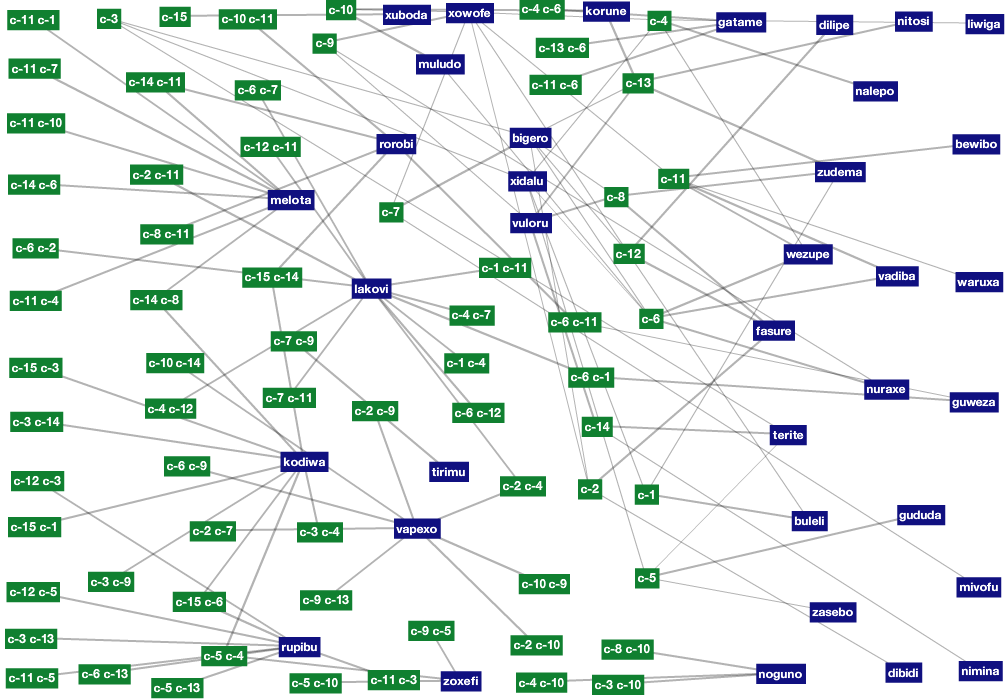
\includegraphics[width=\textwidth]{figures/sgg-mw-structured-lexicon-500}
  \caption{Network representation of the complete lexicon of the first
    agent in the population after 500 interactions. Each line
    represents a word in the lexicon of the agent and connects the
    meaning of the word with its form. The line widths denote the
    strength of the association. }
  \label{f:sgg-mw-structured-lexicon-500}
\end{figure}

\startfiguregroup


\begin{figure}[t]
  \gnuplotfigure{figures/sgg-mw-structured-word-meaning-scores-gesino}
  \caption{Evolution of words with the form ``gesino'' in the
    population. Each line shows for a single meaning the corresponding
    word scores averaged over all agents that associate this meaning
    to ``gesino''. }
  \label{f:sgg-mw-structured-word-meaning-scores-gesino}
\end{figure}

\begin{figure}[t]
  \gnuplotfigure{figures/sgg-mw-structured-word-meaning-scores-xiziwo}
  \caption{Evolution of words with the form ``xiziwo'' in the
    population. }
  \label{f:sgg-mw-structured-word-meaning-scores-xiziwo}
\end{figure}

\stopfiguregroup


Figure \ref{f:sgg-mw-structured-lexicon-500} displays the complete
lexicon of a single agent after 500 interactions. It nicely
illustrates the high number of meanings connected to single forms and
also the high number forms connected to some meanings. In order to
reduce this ambiguity, words need to be tried out in many different
context so that competing forms and meanings can be eliminated through
lateral inhibition. Two typical competition dynamics are given in
Figures \ref{f:sgg-mw-structured-word-meaning-scores-gesino} and
\ref{f:sgg-mw-structured-word-meaning-scores-xiziwo}. The first plots
all the different meanings associated by all the agents in the
population to the form ``gesino'' with their average association
scores. The meaning that eventually wins at around interaction 10000
is \texttt{c-11}, but in the process 36 other competing meanings get
adopted and need to be eliminated. 

A much more typical evolution of a word form is shown in Figure
\ref{f:sgg-mw-structured-word-meaning-scores-xiziwo}. Here, the form
``xiziwo'' attracted 18 different meanings that one after the other
decrease in score until it finally disappears from the population at
around interaction 5500.

~\\

\startfiguregroup

\begin{figure}[t]
  \gnuplotfigure{figures/sgg-mw-structured-success+lexicon-size}
  \caption{Main measures of alignment. Communicated success (measure
    \ref{m:communicative-success}) and lexicon size (measure
    \ref{m:lexicon-size}) are averaged over 10 repeated series of 16000
    language games.}
  \label{f:sgg-mw-structured-success+lexicon-size}
\end{figure}


\begin{figure}[t]
  \gnuplotfigure{figures/sgg-mw-structured-lexicon}
  \caption{Evolution of lexicon structure. The average number of forms
    per meaning (measure \ref{m:synonymy}), the number of meanings per
    form (measure \ref{m:homonymy}), lexicon coherence (measure
    \ref{m:lexicon-coherence} and stability (measure
    \ref{m:frequency-of-lexicon-changes}) are averaged over 10
    repeated series of 16000 interactions.}
  \label{f:sgg-mw-structured-lexicon}
\end{figure}


\stopfiguregroup

The overall dynamics in populations using these kinds of lexicon
representations and learning strategies are given in Figures
\ref{f:sgg-mw-structured-success+lexicon-size} and
\ref{f:sgg-mw-structured-lexicon} and the look very similar to the
ones in the the same diagram for agents using unstructured meanings
from the previous section (see Figures
\ref{f:sgg-mw-unstructured-success+lexicon-size} and
\ref{f:sgg-mw-unstructured-lexicon} on page
\pageref{f:sgg-mw-unstructured-success+lexicon-size}). Complete
communicative success is reached after about 5000 interactions and the
evolution of lexicon size shows the typical shape where first a high
number of words become evented before later alignment reduces many of
them again. 

For reasons that we will briefly discuss in Section
\ref{s:bias-toward-atomic-word-meanings} below, the number of words in
the lexicons of each agent converges to 15, which is also the total
number of categories in the simulated world. Consequently, the average
number of meanings per form and the average number of forms per
meaning also converge to one. The increased ambiguity shows in the
maximum lexicon size of about 160 words that each agent has in its
inventory at around interaction 2000 (compared to about 60 in Figure
\ref{f:sgg-mw-unstructured-lexicon}), a much slower increasing
lexicon coherence and much longer sustained high frequencies of
lexicon changes.


\begin{figure}[t]
  \gnuplotfigure{figures/sgg-mw-structured-misunderstandings+conceptualizations+utterance-length}
  \caption{Causes for ambiguity. The fraction of interactions in which
    communicative success is reached although the speaker and hearer
    used different meanings (measure
    \ref{m:succeeded-with-different-meanings}), the number of
    conceptualizations (measure \ref{m:number-of-conceptualizations})
    and average utterance length (measure \ref{m:utterance-length})
    are averaged over 10 repeated series of 16000 language games.}
  \label{f:sgg-mw-structured-misunderstandings+conceptualizations+utterance-length}
\end{figure}

Some of the challenges that lead to these high uncertainties are
uncertainties in Figure
\ref{f:sgg-mw-structured-misunderstandings+conceptualizations+utterance-length}. The
average number different meanings that can be used to discriminate a
topic from the other objects in the scene is about 4 (because the
world does not change during an experimental run). Furthermore, agents
will communicate successfully while having different understandings of
the meanings in more that 5 percent of the cases during the first 2000
interactions. In this interactions they will wrongly increase the
association scores of the words, while reducing the scores of
competing combinations. And finally, the average utterance length
starts at 1 (the first that speakers will invent cover the complete
uncovered meaning) and gradually converges to 1.5 at around
interaction 2000.


\begin{measure}[b]{Average utterance length}{m:utterance-length}
  Measures the average utterance length, i.e. the number of different
  word forms contained in the utterance produced by the
  speaker. Values are averaged over the last 250 interactions.
\end{measure}


\subsection{The limits of random search}
\label{s:sgg-mv-structured-scaling}

The simulation parameters that were used for the experiments
throughout this chapter are more or less standard in the body of
research that has been done on language game experiments in simulated
environments. The size of the population is 10 agents, simulated world
perceptions consist of two to five objects, each characterized by 10
categories out of an overall fixed set of 15 categories. However, when
increasing the complexity of the scenario slightly beyond these
values, then the strategy of keeping high number of hypotheses of what
words mean in the lexicons of the agents turns out to be a strong
limitation for scaling up. We now briefly analyze the scaling behavior
for increasing population sizes and context sizes.


\startfiguregroup

\begin{figure}[p]
  \gnuplotfigure{figures/sgg-mw-structured-best-best-population-size-vs-lexicon-size}
  \caption{Lexicon size (measure \ref{m:lexicon-size}) for five
    different population sizes. Results are averaged over 10 series of
    varying length, but each with 16000 interactions per agent.}
  \label{f:sgg-mw-structured-best-best-population-size-vs-lexicon-size}
\end{figure}


\begin{figure}[p]
  \gnuplotfigure{figures/sgg-mw-structured-best-best-population-size-vs-lexicon-changes}
  \caption{Frequency of lexicon changes (measure
    \ref{m:frequency-of-lexicon-changes}) for five different population
    sizes. Results are averaged over 10 series of varying length, but
    each with 16000 interactions per agent.}
  \label{f:sgg-mw-structured-best-best-population-size-vs-lexicon-changes}
\end{figure}


\begin{figure}[p]
  \gnuplotfigure{figures/sgg-mw-structured-best-best-population-size-vs-communicative-success}
  \caption{Communi\-cative success (measure
    \ref{m:communicative-success}) for five different population
    sizes. Results are averaged over 10 series of varying length, but
    each with 16000 interactions per agent.}
  \label{f:sgg-mw-structured-best-best-population-size-vs-communicative-success}
\end{figure}

\stopfiguregroup

~\\

The Figures
\ref{f:sgg-mw-structured-best-best-population-size-vs-lexicon-size},
\ref{f:sgg-mw-structured-best-best-population-size-vs-lexicon-changes}
and
\ref{f:sgg-mw-structured-best-best-population-size-vs-communicative-success}
compare lexicon size, frequency of lexicon changes and communicative
success for populations of 10 to 100 agents. In order to be able to
compute these graphs within the memory and computing time limits of
contemporary computer hardware, speakers and hearers use the ``process
1'' respectively ``adopt 1'' strategy for handling alternative
conceptualizations and for adopting word meanings (see page
\pageref{f:sgg-sw-unstructured-50-attrs-conceptualization-handling-vs-lexicon-changes}
et sqq.).

For all five different population sizes, the agents managed to reach
the ``optimal'' lexicon size of 15 words, a stable lexicon that does
not change anymore, and 100\% communicative success. However, reaching
success and coherence takes prohibitively long and agents have to make
huge efforts to align with each other. The average maximum lexicon
size in populations of 100 agents is around 700 words, almost 50 times
as much as the final lexicon size of 15 words. Each agent adds or
removes a word to / from his lexicon in more than 80\% of his first
7000 interactions. And only every tenth out of the first 5000
interactions succeeds. 

It is fair to say that although all involved measures converge, the
alignment strategy of memorizing and later eliminating words does not
scale at all with increasing population size. Agents have to go
through long periods of random search until some words start being
successfully used by a critical fraction of the population. The high
variance across different experimental runs for population sizes above
25 (indicated by the error bars in Figures
\ref{f:sgg-mw-structured-best-best-population-size-vs-lexicon-size},
\ref{f:sgg-mw-structured-best-best-population-size-vs-lexicon-changes}
and
\ref{f:sgg-mw-structured-best-best-population-size-vs-communicative-success})
supports this. In some runs, this ``critical'' moment is reached much
earlier than in others, suggesting that random factors play an
important role in these dynamics. For the case of the Naming Game,
\cite{baronchelli06sharp} have characterized this phenomenon as a
``sharp transition'' from an unordered to an ordered state.

~\\

\startfiguregroup

\begin{figure}[t]
  \gnuplotfigure{figures/sgg-mw-structured-best-best-context-size-vs-number-of-conceptualizations}
  \caption{Number of alternative conceptualizations per scene (measure
    \ref{m:number-of-conceptualizations}) for world simulators with
    increasing number of objects per scene.}
  \label{f:sgg-mw-structured-best-best-context-size-vs-number-of-conceptualizations}
\end{figure}

\begin{figure}[t]
  \gnuplotfigure{figures/sgg-mw-structured-context-size-vs-meaning-length}
  \caption{Average meaning length (measure \ref{m:meaning-length}) for
    world simulators with increasing number of objects per scene.}
  \label{f:sgg-mw-structured-context-size-vs-meaning-length}
\end{figure}

\stopfiguregroup

\begin{measure}[b]{Average meaning length}{m:meaning-length}
  Measures the average meaning length, i.e. the number categories
  contained in the meaning that was conceptualized speaker and used in
  production. Values are averaged over the last 250 interactions.
\end{measure}


For challenging the model with an increasing complexity of the world,
it is enough to increase the number of objects that speakers and
hearers perceive in a single interaction. We chose context size
parameters in such a way that the average number of ways to
conceptualize a scene (and thus the referential uncertainty) stays
more or less the same. Starting from the standard condition in this
chapter in which contexts consisting of 2 to 5 objects, to contexts
with between 5 and 8 objects, there are on average around four
alternative conceptualizations per scene (see Figure
\ref{f:sgg-mw-structured-best-best-context-size-vs-number-of-conceptualizations}).

\startfiguregroup

\begin{figure}[p]
  \gnuplotfigure{figures/sgg-mw-structured-best-best-context-size-vs-lexicon-size}
  \caption{Lexicon size (measure \ref{m:lexicon-size}) for world
    simulators with increasing number of objects per scene. Results
    are averaged over 10 series of 80000 interactions. }
  \label{f:sgg-mw-structured-best-best-context-size-vs-lexicon-size}
\end{figure}


\begin{figure}[p]
  \gnuplotfigure{figures/sgg-mw-structured-best-best-context-size-vs-lexicon-changes}
  \caption{Frequency of lexicon changes (measure
    \ref{m:frequency-of-lexicon-changes}) for world simulators with
    increasing number of objects per scene. Results are averaged over
    10 series of 80000 interactions. }
  \label{f:sgg-mw-structured-best-best-context-size-vs-lexicon-changes}
\end{figure}

\begin{figure}[p]
  \gnuplotfigure{figures/sgg-mw-structured-best-best-context-size-vs-communicative-success}
  \caption{Communi\-cative success (measure
    \ref{m:communicative-success}) for world simulators with
    increasing number of objects per scene. Results are averaged over
    10 series of 80000 interactions. }
  \label{f:sgg-mw-structured-best-best-context-size-vs-communicative-success}
\end{figure}

\stopfiguregroup


Nevertheless, a higher number of objects in a context means that more
categories are needed to discriminate a topic from the other objects
in the context, which is illustrated in Figure
\ref{f:sgg-mw-structured-context-size-vs-meaning-length}. The average
number of categories that speakers need to conceptualize a scene rises
from about 1.5 in contexts of 2 to 5 objects to about 2.2 in contexts
with 5 to 8 objects (see Figure
\ref{f:sgg-mw-structured-context-size-vs-meaning-length}).

This small increase complexity causes a drastic increase in the amount
of work that agents have to do in order to keep track of word
meanings, leading to an even worse scaling behavior than with
population size (see Figures
\ref{f:sgg-mw-structured-best-best-context-size-vs-lexicon-size},
\ref{f:sgg-mw-structured-best-best-context-size-vs-lexicon-changes}
and
\ref{f:sgg-mw-structured-best-best-context-size-vs-communicative-success}). Only
for the first two world simulator configurations (perceived contexts
consist of between 2 and 5 objects, respectively 2 and 6 objects) the
population of again 10 agents is able to reach complete success and
lexicon stability. The high variance indicated by the error bars
across different runs for contexts with between 3 and 6 objects
indicates that in this case the population was able to converge in
some of the runs whereas in others not. Anyway, for all other
configurations, the lexicon representation and the strategies for
alignment simply don't work.



\subsection{Bias towards atomic word meanings}
\label{s:bias-toward-atomic-word-meanings}

Although the agents are endowed with the capacity to represent and
process compositional word meanings, the lateral inhibition dynamics
used by the agents to gradually reduce alternative hypotheses
constitute a bias towards unstructured word meanings. 

\startfiguregroup

\begin{figure}[t]
  
{\footnotesize\renewcommand{\arraystretch}{1.5}
\begin{tabular}{@{}p{1.2cm}|p{1.6cm}@{}p{0.8cm}@{}|p{1.6cm}@{}p{0.8cm}@{}|p{1.6cm}@{}p{0.8cm}@{}|p{1.6cm}@{}p{0.8cm}@{}}
meaning & agent 1 &  & agent 2 &  & agent 3 &  & agent 4 & \\
\hline
\texttt{c-1}&\textit{``vepolu''}
&1.00&\textit{``vepolu''}
&1.00&\textit{``vepolu''}
&1.00&\textit{``vepolu''}
&1.00\\
\hline
\texttt{c-2}&\textit{``letibe''}
&1.00&\textit{``letibe''}
&1.00&\textit{``letibe''}
&1.00&\textit{``letibe''}
&1.00\\
\hline
\texttt{c-1 c-2}&\textit{``beleno''}

\textit{``zifuxa''}
&0.10

0.10&\textit{``suloko''}
&0.20&&&&
\end{tabular}}

  \caption{Forms associated to 3 different meanings by the first four
    agents of a population of 10 after 5000 interactions.}
  \label{f:sgg-mw-structured-lexicon-meanings-5000}
\end{figure}

\begin{figure}[t]
  
{\renewcommand{\arraystretch}{1.5}
\begin{tabular}{@{}p{1.2cm}|p{1.6cm}@{}p{0.8cm}@{}|p{1.6cm}@{}p{0.8cm}@{}|p{1.6cm}@{}p{0.8cm}@{}|p{1.6cm}@{}p{0.8cm}@{}}
form & agent 1 &  & agent 2 &  & agent 3 &  & agent 4 & \\
\hline
\textit{``xavuto''}&\texttt{c-8}
&0.50&\texttt{c-8}
&0.70&\texttt{c-8}
&0.30&\texttt{c-8}
&0.60\\
\hline
\textit{``buxoxo''}&\texttt{c-8}
&0.10&\texttt{c-8}
&0.10&&&&\\
\hline
\textit{``vewuxa''}&\texttt{c-13}
&1.00&\texttt{c-13}
&1.00&\texttt{c-13}
&1.00&\texttt{c-13}
&1.00\\
\hline
\textit{``vaxutu''}&\texttt{c-3 c-12}
&1.00&\texttt{c-3}
&1.00&\texttt{c-3}
&1.00&\texttt{c-3}
&1.00\\
\hline
\textit{``godefe''}&\texttt{c-11 c-8}


\texttt{c-13 c-8}


\texttt{c-13 c-3}
&0.30

0.50

0.50&\texttt{c-14 c-9}


\texttt{c-2 c-14}
&0.30

0.30&&&\texttt{c-13 c-6}
&0.20\\
\end{tabular}}

  \caption{Meanings associated to 3 different forms by the first four
    agents of a population of 10 after 5000 interactions.}
  \label{f:sgg-mw-structured-lexicon-forms-5000}
\end{figure}

\stopfiguregroup

The lexicon snapshots of the same four agents from Figures
\ref{f:sgg-mw-structured-lexicon-meanings-1500} and
\ref{f:sgg-mw-structured-lexicon-forms-1500} but 3500 interactions
later at interaction 5000 (Figures
\ref{f:sgg-mw-structured-lexicon-meanings-5000} and
\ref{f:sgg-mw-structured-lexicon-forms-5000}) illustrate this. All
four agents agreed on the same forms ``vepolu'' and ``letibe'' for the
atomic meanings \texttt{c-1} and \texttt{c-2} and all converged to the
highest score of 1.0 for these associations. On the contrary, there is
no conventionalized form for the structured meaning \texttt{c-1 c-2}
and the three words that remained in the population have very low
association scores. Looking form the other direction, word forms that
are connected to single categories are so with higher scores than
those that map to structured meanings. An interesting and rare
exception is the form ``vaxutu''. While all other agents connect the
meaning \texttt{c-3} to it, the first agent uses the two categories
\texttt{c-3 c-12}.


The explanation for this effect is something that
\cite{debeule06compositionality} called a frequency effect. Lateral
inhibition after a successful language game operates equally on all
words that also could have been applied, and consequently words
connected to single categories have an advantage in these dynamics. In
the example above, the words expression the category combination
\texttt{c-1 c-2} are in direct competition with the words expressing
\texttt{c-1} or \texttt{c-2} for all conceptualizations that contain
these two categories. However, words expressing \texttt{c-1 c-2} can
only be used in such situations, whereas words expressing single
categories can be used in a much wider variety of contexts (basically
all conceptualizations that contain that category). They thus can be
tried out more frequently, and consequently can spread more quickly
the population and be part of more successful interactions. Which
means that they will have higher combined scores than their structured
counterparts and finally win the competition over them.



% %%% Local Variables: 
% %%% mode: latex
% %%% TeX-master: "phdbook"
% %%% End: 
